% !BIB program = bibtex
\documentclass[12pt]{article}

%----------------------------------------------------------------------------------------
%	FONTS
%----------------------------------------------------------------------------------------

% Required for inputting international characters
\usepackage[T1]{fontenc}

% Use 8-bit encoding
\usepackage[latin1,utf8]{inputenc}

% Fonts
\usepackage{lmodern}

%----------------------------------------------------------------------------------------
%	PACKAGES AND OTHER DOCUMENT CONFIGURATIONS
%----------------------------------------------------------------------------------------

% Generate dummy text (lorem ipsum) in your document
\usepackage{lipsum} % Comment me

% English language hyphenation
\usepackage[portuguese]{babel}

% Math packages
\usepackage{amsmath, amsfonts, amsthm}

% Indent first paragraph
\usepackage{indentfirst}

% Spacing
% \setlength{\parskip}{0.2cm}  % tente também \onelineskip
% \setlength{\parindent}{2cm}
\usepackage{setspace}
\doublespacing
\frenchspacing

% Figures
\usepackage{float}
\usepackage{graphicx}
\graphicspath{{./images/}}

% Bold font for Tabela and Figura
\addto\captionsportuguese{
  \renewcommand{\tablename}{\bfseries Tabela}
  \renewcommand{\figurename}{\bfseries Figura}
}

% TikZ UML diagrams
\usepackage{tikz}
\usepackage{tikz-uml}

% Captions
\usepackage{caption}
\usepackage{subcaption}

% Tables
\usepackage{tabularx}
\usepackage{pgfgantt}

% PGFPlots
\usepackage{pgfplots}
\pgfplotsset{compat=1.18}

% Header and footer
\usepackage{fancyhdr}

% Table of contents
\usepackage{tocloft}
% Dots for sections
\renewcommand{\cftsecleader}{\cftdotfill{\cftdotsep}}
% Center the table of contents title
\addto\captionsportuguese{
  \renewcommand{\contentsname}{\hfill\bfseries\Large Sumário \hfill}
  \renewcommand{\cftaftertoctitle}{\hfill}
}

% Context sensitive quotation facilities
\usepackage{csquotes}

% Enumerate
\usepackage[inline]{enumitem}

% Chemical formulas package
\usepackage{chemformula}

% Shorthands
\usepackage{xspace}

% Code highlighting
\usepackage{minted}

% PDF
\usepackage{pdfpages}

% Tables
\usepackage{booktabs}
\usepackage{tabularx}

% Array package
\usepackage{array}

% URL package
\usepackage[hyphens]{url}

% Microtypography
\usepackage{microtype}

% Adjustbox for image positioning
\usepackage[export]{adjustbox}

\makeatletter
\def\eg{e.g\onedot} \def\Eg{E.g\onedot}
\def\ie{i.e\onedot} \def\Ie{I.e\onedot}
\def\cf{cf\onedot} \def\Cf{Cf\onedot}
\def\etc{etc\onedot} \def\vs{vs\onedot}
\def\wrt{w.r.t\onedot} \def\dof{d.o.f\onedot}
\def\etal{et al.\onedot}
\makeatother

% Hyperlinks styling
\usepackage{hyperref}
% Hyperlink setup
\hypersetup{
  colorlinks   = true, % Colours links instead of ugly boxes
  urlcolor     = blue, % Colour for external hyperlinks
  linkcolor    = blue, % Colour of internal links
  citecolor    = blue, % Colour of citations
  linktocpage  = true, % Link only on page numbers
}
% PDF metadata
\hypersetup{
  pdftitle     = {Implementação de protocolo de processamento de
  imagens em ensaios fenotípicos de viabilidade celular},
  pdfauthor    = {Kayllany Oliveira, João VS Guerra},
  pdfproducer  = {Latex with hyperref},
  pdfcreator   = {pdflatex}
}

% Bibliography
\usepackage[num,abnt-etal-text=emph,bibjustif]{abntex2cite}
\usepackage{cite}
\renewcommand\citeleft{[}
\renewcommand\citeright{]}

% Acronyms
\usepackage[
  printonlyused,
  nohyperlinks,
  withpage,
]{acronym}

% Directory tree
\usepackage{dirtree}

%----------------------------------------------------------------------------------------
%	DOCUMENT MARGINS
%----------------------------------------------------------------------------------------

\usepackage{geometry} % Required for adjusting page dimensions and margins
\geometry{
    paper=a4paper,
    top=30mm, % Top margin
    bottom=20mm, % Bottom margin
    left=30mm, % Left margin
    right=20mm, % Right margin
    % showframe, % Uncomment to show how the type block is set on the page
}

%----------------------------------------------------------------------------------------
% DOCUMENT
%----------------------------------------------------------------------------------------

\begin{document}

% Title Page
\begin{titlepage}
  % Logo
  \begin{center}
      \begin{minipage}{\textwidth}%
      
\includegraphics[width=\textwidth]{lnbio-cnpem-logo.png}%
      \end{minipage}
  \end{center}

  \vskip 0.5cm

  % Title
  {\centering \large \bfseries Implementação de protocolo de processamento de imagens em ensaios fenotípicos de viabilidade celular \par}

  \vskip 1.5cm

  % Funding
  \hline
  \vskip 1.0cm
  {\centering \normalsize Relatório Científico Final de Bolsas no País de Iniciação Científica, fomentado pela Fundação de Amparo à Pesquisa do Estado de São Paulo (FAPESP) \par}
  \vskip 1.0cm
  \hline

  \vskip 1.0cm

  \begin{center}
    \normal Processo FAPESP \#2025/05515-6\par
    \vskip 0.5cm
    \normal \textbf{Bolsista:} Kayllany Lara da Silva Oliveira\par
    \normal \textbf{Orientador:} Dr. João Victor da Silva Guerra\par
    \normal \textbf{Coorientador:} Dr. José Geraldo de Carvalho Pereira \par
    \normal \textbf{Coorientadora:} Dra. Ana Amélia Sanchez Iacia \par
  \end{center}

  \vskip 2.0cm
  {\centering \normal Laboratório Nacional de Biociências - LNBio \par}
  {\centering \normal Centro Nacional de Pesquisa em Energia e Materiais - CNPEM \par}

  % Date
  \vfill
  \begin{center}
    \normal Campinas, 10 Janeiro de 2026\par
  \end{center}

\end{titlepage}

%% Informações Gerais do Projeto
\section*{\center Informações Gerais do Projeto}

\addcontentsline{toc}{section}{Informações Gerais do Projeto}

\begin{itemize}
  \item \textbf{Título do projeto:} Implementação de protocolo de processamento de imagens em ensaios fenotípicos de viabilidade celular
  \item \textbf{Número do projeto de pesquisa:} 2025/05515-6
  \item \textbf{Período de vigência:} 01/06/2025 a 31/12/2025
  \item \textbf{Período coberto por este relatório científico:} 01/06/2025 a 31/12/2025
\end{itemize}

\clearpage

% Table of Contents
\tableofcontents
\pagebreak

\section{Resumo do projeto proposto}

A microscopia óptica, em especial a microscopia por fluorescência, é uma ferramenta central nas ciências da vida, permitindo a visualização detalhada de estruturas celulares e a extração de informações quantitativas a partir de imagens biológicas. Nesse contexto, a triagem automatizada de alto rendimento (do inglês, \textit{High-Throughput Screening}; HTS) e de alto conteúdo (do inglês, \textit{High-Content Screening}; HCS) integra microscopia automatizada e análise computacional para a avaliação sistemática de milhares de compostos em microplacas, sendo amplamente aplicada em biologia celular, virologia e descoberta de fármacos. Entretanto, o grande volume e a complexidade dos dados gerados impõem desafios relevantes de escalabilidade computacional, reprodutibilidade e custo, especialmente quando as análises dependem de softwares proprietários pouco flexíveis e de difícil integração com infraestruturas de computação de alto desempenho.

Para enfrentar esses desafios, este projeto desenvolveu um protocolo computacional automatizado e de código aberto para o processamento e a análise de imagens de ensaios fenotípicos de viabilidade celular. O protocolo foi implementado como um pacote em Python, denominado \texttt{CellViability}, projetado para ser reprodutível, escalável e compatível com ambientes de computação de alto desempenho.

O pacote \texttt{CellViability} foi desenvolvido na Equipe de Dados Biológicos (EDB) do LNBio/CNPEM, a partir de dados gerados pelo Laboratório de Bioensaios (LBE). As imagens foram adquiridas em placas de 384 poços no sistema de microscopia automatizada \textit{Operetta CLS High-Content Analysis System} (Perkin Elmer), com marcação nuclear com o fluoróforo Hoechst 33342. Os ensaios envolveram linhagens celulares Vero CCL81 e HuH7.0 infectadas com diferentes vírus, incluindo Mayaro (MAYV), SARS-CoV-2, Oropouche (OROV) e vírus da encefalite de St. Louis (SLEV), no contexto de campanhas de descoberta de fármacos antivirais.

O protocolo foi estruturado em etapas bem definidas, incluindo carregamento das imagens, segmentação dos núcleos celulares, extração de características morfológicas e contagem celular por poço, normalização dos dados pelo índice de inibição do efeito citopático (inCPE), controle de qualidade das placas com o fator $Z'$, visualização dos resultados e integração dos dados para seleção de compostos candidatos.

A segmentação celular foi avaliada com modelos baseados em aprendizado profundo, incluindo Cellpose (v3.1.1.2 e v4.0.7) e StarDist (v0.9.1), sendo este último o que apresentou melhor desempenho global, com alta concordância em relação ao método comercial de referência e menor custo computacional. Após a segmentação, a contagem de núcleos foi utilizada como métrica primária de viabilidade celular, e os dados foram normalizados pelo cálculo do inCPE, permitindo comparações diretas entre poços e placas. O controle de qualidade foi realizado com base no fator $Z'$, assegurando que apenas placas com desempenho estatístico adequado fossem incluídas nas análises subsequentes. Os dados aprovados foram integrados em nível de \textit{screening}, organizados em estruturas tabulares e exportados em formatos amplamente utilizados. As visualizações geradas incluem sobreposições das segmentações sobre as imagens originais e mapas de placa, facilitando a interpretação dos resultados.

O \texttt{CellViability} foi disponibilizado como um pacote Python de código aberto, acompanhado de documentação técnica, contribuindo para a adoção de práticas abertas, escaláveis e reprodutíveis na análise de bioimagens em HTS e HCS, com impacto direto em estudos de viabilidade celular e descoberta de fármacos. A futura integração do \texttt{CellViability} à infraestrutura de computação de alto desempenho do LNBio permitirá explorar paralelização a nível de placas ou poços, reduzindo significativamente o tempo de processamento de grandes volumes de imagens em comparação com a solução comercial de referência.

\section{Realizações no projeto}

O projeto foi desenvolvido pela Equipe de Dados Biológicos (EDB), com validação experimental realizada a partir de dados do Laboratório de Bioensaios (LBE) do LNBio, instalação aberta do CNPEM. O processamento das imagens biológicas da triagem automatizada foi realizado no cluster de computação de alto desempenho do LNBio, denominado de HPCC Marvin, composto por 2 nós de processamento com 128 núcleos e 2 TB RAM, sendo que um deles possui 8 GPUs NVIDIA A100 (40GB), além do servidor de desenvolvimento com 48 núcleos, 256 GB RAM e 1 GPU NVIDIA RTX 3070 (8GB).

\subsection{Imagens biológicas}

As imagens de fluroescência dos ensaios de viabilidade celular foram fornecidas pelo grupo de Virologia do LNBio/CNPEM, liderado pelo Dr. Rafael Elias Marques. As aquisições foram realizadas em placas de 384 poços, usando o sistema de microscopia \textit{Operetta CLS High-Content Analysis System} (Perkin Elmer), com magnificação de 10x, capturando o campo central de cada poço.

Os experimentos envolveram a infecção das linhagens Vero CCL81 e HuH7.0 com os vírus Mayaro (MAYV), coronavírus da síndrome respiratória aguda grave 2 (SARS-CoV-2), Oropouche (OROV) e vírus da encefalite de St. Louis (SLEV). As células Huh-7 foram expostas a 7.784 compostos contra MAYV, OROV e SLEV, enquanto as células Vero CCL81 foram testadas com 3.212 compostos contra SARS-CoV-2. As células foram estocados em 100\% DMSO, além de controles não infectados (negativo) e infectados (positivo), ambos sem tratamento. Todas as amostras, incluindo controles, continham 0,4\% de DMSO. A coloração celular foi realizada com o fluoróforo Hoechst 33342, um marcador de DNA, permitindo a segmentação dos núcleos celulares. A aquisição das imagens foi feita utilizando um filtro de excitação a 361 nm e emissão a 497 nm.

\subsection{Desenvolvimento do protocolo de processamento de imagens em ensaios de viabilidade celular}

O protocolo computacional de processamento de imagens em ensaios de viabilidade celular para descoberta de fármacos foi implementado como um pacote de código aberto denominado \texttt{CellViability}, desenvolvido em Python e licenciado sob a licença GPL 3.0. Para isso, foram usadas bibliotecas de código aberto para leitura, pré-processamento, segmentação e caracterização de imagens biológicas, incluindo BioIO \cite{bioio}, scikit-image \cite{vanderWalt2014}, scipy.ndimage \cite{Virtanen2020}, Cellpose \cite{Stringer2020,Stringer2025,Pachitariu2025} e StarDist \cite{Schmidt2018,Weigert2020,Weigert2022}.

O protocolo foi estruturado em etapas principais:
\begin{enumerate*}[label=(\arabic*)]
  \item carregamento das imagens dos ensaios com \textit{lazy-loading};
  \item segmentação dos núcleos e extração de características morfológicas;
  \item normalização dos dados;
  \item controle de qualidade das placas;
  \item visualização dos dados das placas;
  \item integração dos dados de diferentes placas e seleção dos compostos candidatos.
\end{enumerate*}

A partir dessas etapas, a arquitetura do pacote foi organizada em três subpacotes principais (Figura \ref{fig:cv-uml}): \texttt{protocols}, \texttt{screening} e \texttt{core}.

\begin{figure}[H]
  \begin{center}
    \begin{tikzpicture}[scale=0.42, every node/.style={transform shape, inner sep=0pt}]

      \begin{umlpackage}{CellViability}

        \begin{umlpackage}[x=-2, y=0]{protocols}

          \umlclass[x=0, y=0, width=120ex]{CellViabilityProtocol}{
            +config : dict[str, any] \\
            +name : str \\
            +screen : Screen
          }{
            \umlvirt{\texttt{\string-}\_load\_model(warmup: bool) : StarDist2D} \\
            \umlvirt{\texttt{\string-}\_load\_screen(config) : Screen} \\
            \umlvirt{\texttt{\string-}\_segment(image : Image, channel : int, **kwargs) : Image} \\
            \umlvirt{\texttt{\string-}\_characterize(segmented : Image) : pandas.DataFrame} \\
            \umlvirt{\texttt{\string-}\_analyze\_plate(plate : Plate, **kwargs) : (pandas.DataFrame, pandas.DataFrame)} \\
            \umlvirt{\texttt{\string-}\_analyze\_well(plate : Plate, well : Well, **kwargs) : (int, pandas.DataFrame)} \\
            +execute() : (pandas.DataFrame, pandas.DataFrame)
          }

        \end{umlpackage}

        \begin{umlpackage}[x=0, y=-12]{screening}

          \umlclass[x=-10, y=0, width=30ex]{Screen}{
            +config : dict[str, any] \\
            +name : str \\
            +plates : list[Plate]
          }{
            \umlvirt{\texttt{\string-}\_load\_plates(config) : list[Plate]} \\
            +plate(idx : int | str) : Plate
          }

          \umlclass[x=-2, y=0, width=30ex]{Plate}{
            +config : dict[str, any] \\
            +name : str \\
            +datadir : str \\
            +wells : list[Well]
          }{
            \umlvirt{\texttt{\string-}\_load\_wells(config) : list[Well]} \\
            +well(name : str) : Well
          }

          \umlclass[x=7.5, y=0, width=30ex]{Well}{
            +name : str \\
            +images : list[Image]
          }{
            \umlvirt{\texttt{\string-}\_load\_image(filenames : list[str]) : list[Image]} \\
            +image(field : int) : Image
          }

          \umlclass[x=18, y=0, width=40ex]{Image}{
            +name : str \\
            +filename : str \\
            +field : int \\
            \umlvirt{\texttt{\string-}\_image : BioImage}
          }{
            +lazy\_load(field : int, filename : str) : BioImage \\
            +upload(image : BioImage) : void \\
            +data() : numpy.ndarray \\
            +image() : BioImage
          }

        \end{umlpackage}

        \begin{umlpackage}[x=8, y=2.5]{core}

          \umlclass[x=10, y=0, type=module, width=40ex]{cli}{}{
          +cli() : argparse.Namespace \\
          +run() : void
          }

        \end{umlpackage}

      \end{umlpackage}

      \umlunicompo[geometry=|-|,pos1=0.6,pos2=2.8,anchor1=-90,anchor2=90,mult1=1,mult2=1]{CellViabilityProtocol}{Screen}
      \umlunicompo[geometry=-|-,arm1=1.0cm,pos1=1.0,pos2=2.2,anchor1=30,anchor2=-160,mult1=1,mult2=1..*]{Screen}{Plate}
      \umlunicompo[geometry=-|-,arm1=1.2cm,pos1=1.0,pos2=2.3,anchor1=30,anchor2=-160,mult1=1,mult2=1..*]{Plate}{Well}
      \umlunicompo[geometry=-|-,arm1=1.0cm,pos1=1.0,pos2=2.2,anchor1=20,anchor2=-160,mult1=1,mult2=1..*]{Well}{Image}
      \umluniassoc[anchor1=-160,anchor2=20,mult1=1,mult2=1]{cli}{CellViabilityProtocol}

    \end{tikzpicture}
  \end{center}
  \caption{\textbf{Diagrama de classes UML do protocolo \texttt{CellViability}.} O diagrama ilustra a organização modular do pacote e os relacionamentos entre as principais classes envolvidas no processamento de imagens em ensaios fenotípicos de viabilidade celular.}
  \label{fig:cv-uml}
\end{figure}

O subpacote \texttt{protocols} contém a classe \texttt{CellViabilityProtocol}, responsável por estruturar o fluxo de processamento, incluindo leitura dos dados, segmentação de imagens, extração de características, integração dos dados e seleção dos \textit{hits}. O subpacote \texttt{screening} reúne as classes que representam a hierarquia experimental de ensaios de descoberta de fármacos (i.e., \texttt{Screen}, \texttt{Plate}, \texttt{Well} e \texttt{Image}), permitindo organizar e acessar eficientemente os dados brutos de imagem.

O subpacote \texttt{core} contém o módulo \texttt{cli}, que fornece uma interface de linha de comando (CLI) para execução do pacote CellViability para facilitar a execução do protocolo pelos usuários finais (Figura \ref{fig:cli}). Essa CLI facilita o uso do protocolo pelos usuários finais, permitindo configurar e processar um ou mais ensaios de viabilidade celular a partir de um arquivo de configuração no formato JSON (\texttt{config.json}). Quando o arquivo contém múltiplos ensaios, cada um deve possuir seu próprio conjunto de parâmetros. Caso o usuário deseje executar apenas um ensaio específico, deve utilizar a opção \texttt{-{}-index} seguida do índice correspondente (iniciando em zero).

\begin{figure}[ht]
  \begin{minted}[linenos=true, tabsize=4, breaklines]{bash}
  $ CellViability --config config.json --basedir /path/to/output/directory --instances --npy --verbose
  \end{minted}
  \caption{\textbf{Exemplo de comando para execução do protocolo \texttt{CellViability} via CLI.} O comando executa o protocolo usando o arquivo de configuração \texttt{config.json}, salvando os resultados no diretório especificado por \texttt{/path/to/output/directory}. As opções adicionais incluem a geração de imagens de instâncias segmentadas (\texttt{-{}-instances}), salvamento das instâncias segmentadas em formato NumPy (\texttt{-{}-npy}) e ativação do modo verboso (\texttt{-{}-verbose}).}
  \label{fig:cli}
\end{figure}

\subsubsection{Arquivo de configuração}

O arquivo \texttt{config.json} (Figura \ref{fig:json-example}) define os parâmetros do protocolo de processamento dos ensaios de viabilidade celular, possibilitando a adaptação do fluxo de trabalho para diferentes condições experimentais.

\begin{figure}[h]
  \begin{minted}[linenos=true, tabsize=4, fontsize=\footnotesize]{json}
  {
    "MAYV": {
      "controls": {
        "negative": [
          "A01", "B01", "C01", "D01", "E01", "F01", "G01", "H01",
          "I01", "J01", "K01", "L01", "M01", "N01", "O01", "P01",
          "A24", "B24", "C24", "D24", "E24", "F24", "G24", "H24",
          "I24", "J24", "K24", "L24", "M24", "N24", "O24", "P24"
        ],
        "positive": [
          "A02", "B02", "C02", "D02", "E02", "F02", "G02", "H02",
          "I02", "J02", "K02", "L02", "M02", "N02", "O02", "P02",
          "A23", "B23", "C23", "D23", "E23", "F23", "G23", "H23",
          "I23", "J23", "K23", "L23", "M23", "O23", "N23", "P23"
        ]
      },
      "datadir": "data/MAYV/",
      "fields": 1,
      "filter": {"inCPE": 0.3, "Z": 0.5},
      "parameters": {"channel": 0, "sigma": 1.0, "min_size": 0, "max_size": 500,
                    "merge": "sum"},
      "plates": ["M1", "M2", "M3", "M4", "M5", "M6", "M7", "M8", "M9", "M10",
                "M11", "M12", "M13", "M14", "M15", "M16", "M17", "M18",
                "M19", "M20", "M21", "M22", "M23", "M24", "M25"],
      "wells": 384
    }
  }
  \end{minted}
  \caption{\textbf{Exemplo de arquivo de configuração JSON para o protocolo \texttt{CellViability}.} O arquivo define os parâmetros necessários para o processamento do ensaio fenotípico de viabilidade celular para o vírus Mayaro.}
  \label{fig:json-example}
\end{figure}

Os campos configuráveis incluem:

\begin{itemize}
  \item \texttt{controls}: listas de poços correspondentes aos controles negativos (não infectados, sem tratamento) e positivos (infectados, sem tratamento) para cada ensaio;
  \item \texttt{datadir}: diretório raiz onde as imagens do ensaio estão armazenadas, seguindo a estrutura de diretórios especificada;
  \item \texttt{fields}: número de campos de imagem por poço (para os ensaios deste projeto, cada poço contém apenas um campo);
  \item \texttt{filter}: critérios de seleção dos compostos candidato (\textit{hits}), incluindo:
  \begin{itemize}
    \item \texttt{inCPE}: limiar mínimo de inibição do efeito citopático viral para seleção dos compostos candidatos (padrão: 0,3);
    \item \texttt{Z}: limiar mínimo do $Z'$ para aprovação das placas no controle de qualidade (padrão: 0,5).
  \end{itemize}
  \item \texttt{parameters}: parâmetros de pré-processamento, segmentação e mineração, incluindo:
  \begin{itemize}
    \item \texttt{channel}: índice do canal de fluorescência a ser analisado (0 para o canal azul, correspondente ao Hoechst 33342);
    \item \texttt{sigma}: valor do desvio padrão para o filtro Gaussiano aplicado no pré-processamento;
    \item \texttt{min\_size} e \texttt{max\_size}: tamanhos mínimo e máximo dos núcleos segmentados, em pixels, para filtragem;
    \item \texttt{merge}: método de agregação dos campos de imagem por poço (soma).
  \end{itemize}
  \item \texttt{plates}: lista de identificadores das placas a serem analisadas no ensaio;
  \item \texttt{wells}: número total de poços por placa (384 para os ensaios deste projeto).
\end{itemize}

Essa estrutura modular torna o protocolo flexível, permitindo seu uso em diferentes ensaios e facilitando sua integração futura com interfaces gráficas (GUI).

\subsubsection{Carregamento dos dados}

Os ensaios fenotípicos de viabilidade celular são usualmente constituídos por múltiplas placas de 384 poços, sendo que cada poço pode um ou mais campos campos (\textit{fields}). Para os ensaios deste projeto (MAYV, OROV, SARS-CoV-2, SLEV), cada poço contém apenas um campo. As imagens foram exportadas pelo software Acapella/Columbus (PerkinElmer), que adota uma convenção padronizada de nomes de arquivos (\eg, \texttt{001001-1-001001001.tif}), permitindo identificar metadados essenciais diretamente a partir do nome do arquivo. Esses metadados incluem a identificação do poço (\textit{well}), campo (\textit{field}), canal de fluorescência, plano Z e tempo.

A leitura das imagens foi implementada utilizando o conceito de \textit{lazy-loading}, permitindo o carregamento sob demanda e reduzindo o consumo de memória total durante o processamento. As imagens são carregadas apenas no momento do processamento de cada campo, reduzindo o uso de memória RAM, possibilitando um processamento mais eficiente em clusters de computação de alto desempenho, como o HPCC Marvin do LNBio/CNPEM.

\subsubsection{Segmentação dos núcleos}

A segmentação das imagens foi realizada para isolar os núcleos das células Vero CCL81 e HuH7.0, marcados com Hoechst 33342. Para essa etapa, diferentes modelos avançados de reconhecimento de instância foram avaliados, incluindo:

\begin{itemize}
  \item Cellpose 3.1.1.2 \cite{Stringer2020,Stringer2025}
  \item Cellpose 4.0.7 \cite{Pachitariu2025}
  \item StarDist 0.9.1 \cite{Schmidt2018,Weigert2020,Weigert2022}.
\end{itemize}

A avaliação foi realizada utilizando as imagens da placa S1 do ensaio de viabilidade celular empregado na triagem de compostos antivirais contra o vírus da encefalite de St. Louis (SLEV). Na segmentação, os núcleos celulares menores ou maiores que limiares definidos pelo usuário são descartados para evitar contagens incorretas devido a artefatos ou núcleos sobrepostos. Os modelos foram aplicados ao mesmo conjunto de imagens, comparando ao software comercial Acapella/Columbus, referência atual no LNBio. A avaliação foi baseada no seguintes critérios: número de células identificadas, qualidade das segmentações, tempo de processamento e uso de recursos computacionais.

\begin{figure}[h]
  \centering
  \begin{subfigure}[b]{0.325\textwidth}
    \centering
    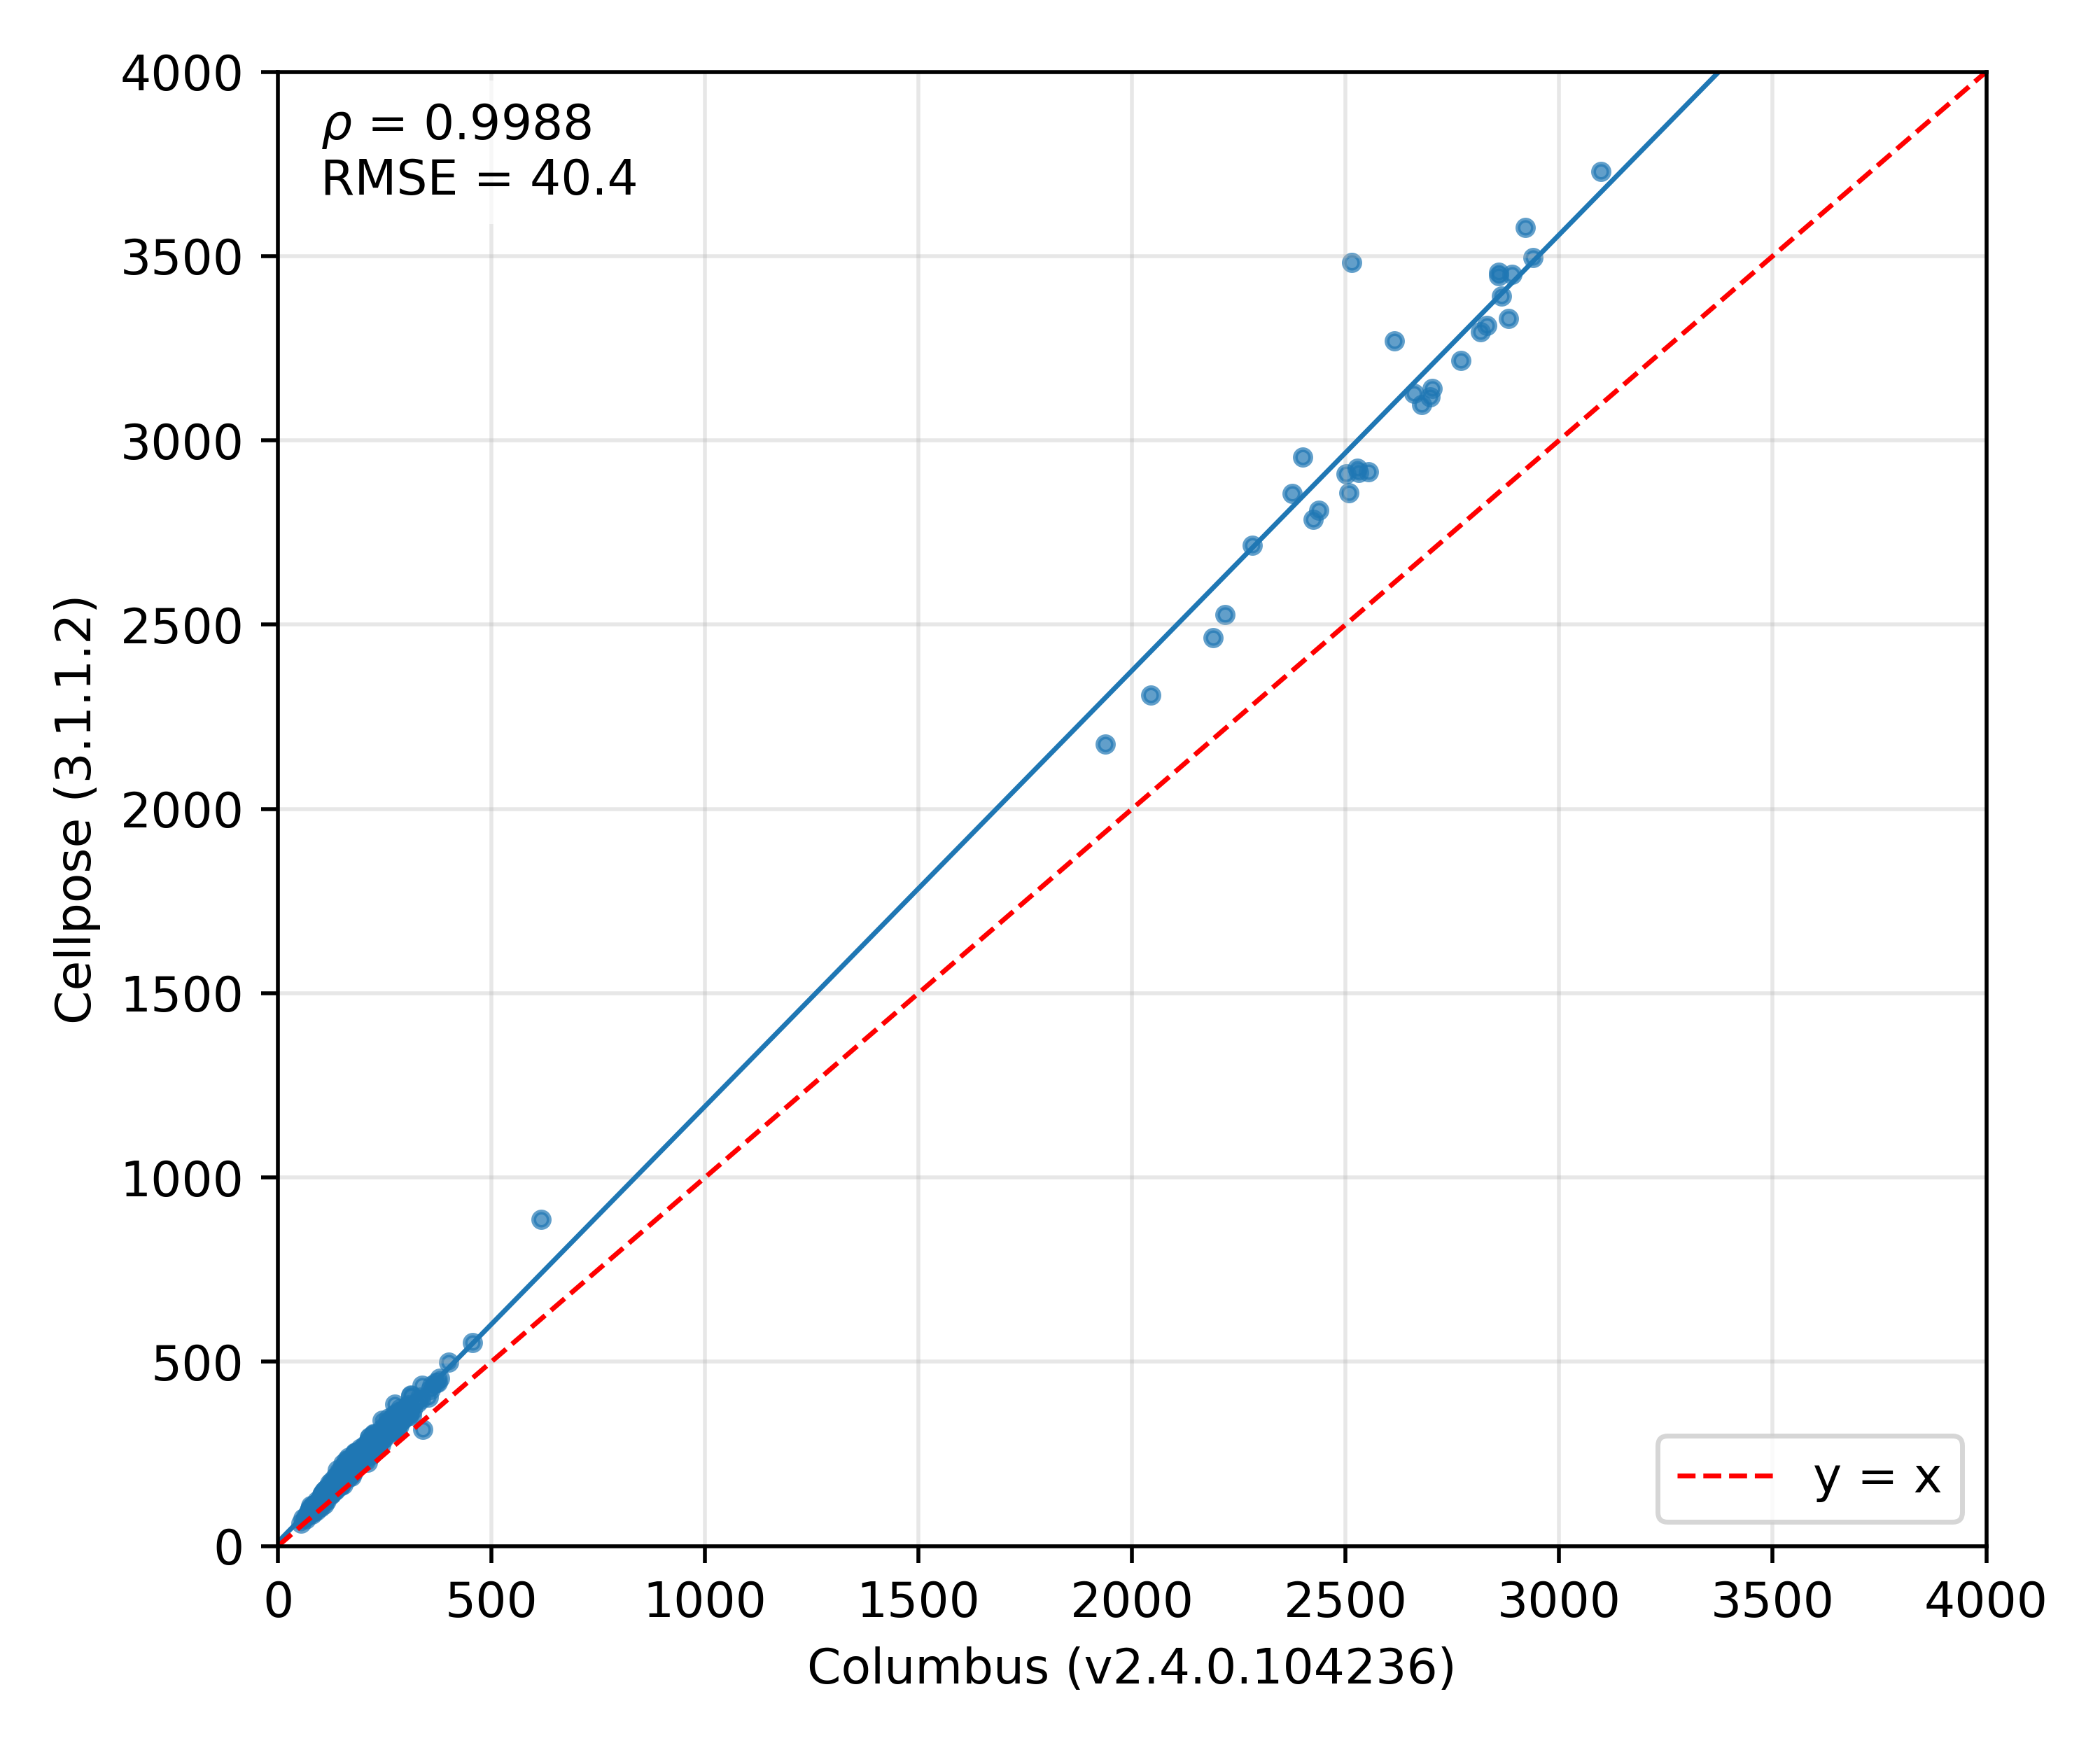
\includegraphics[width=\textwidth]{dispersion/Cellpose_3.1.1.2.png}
    \caption*{(A) Cellpose 3.1.1.2}
    \label{fig:cellpose3112}
  \end{subfigure}
  \hfill
  \begin{subfigure}[b]{0.325\textwidth}
    \centering
    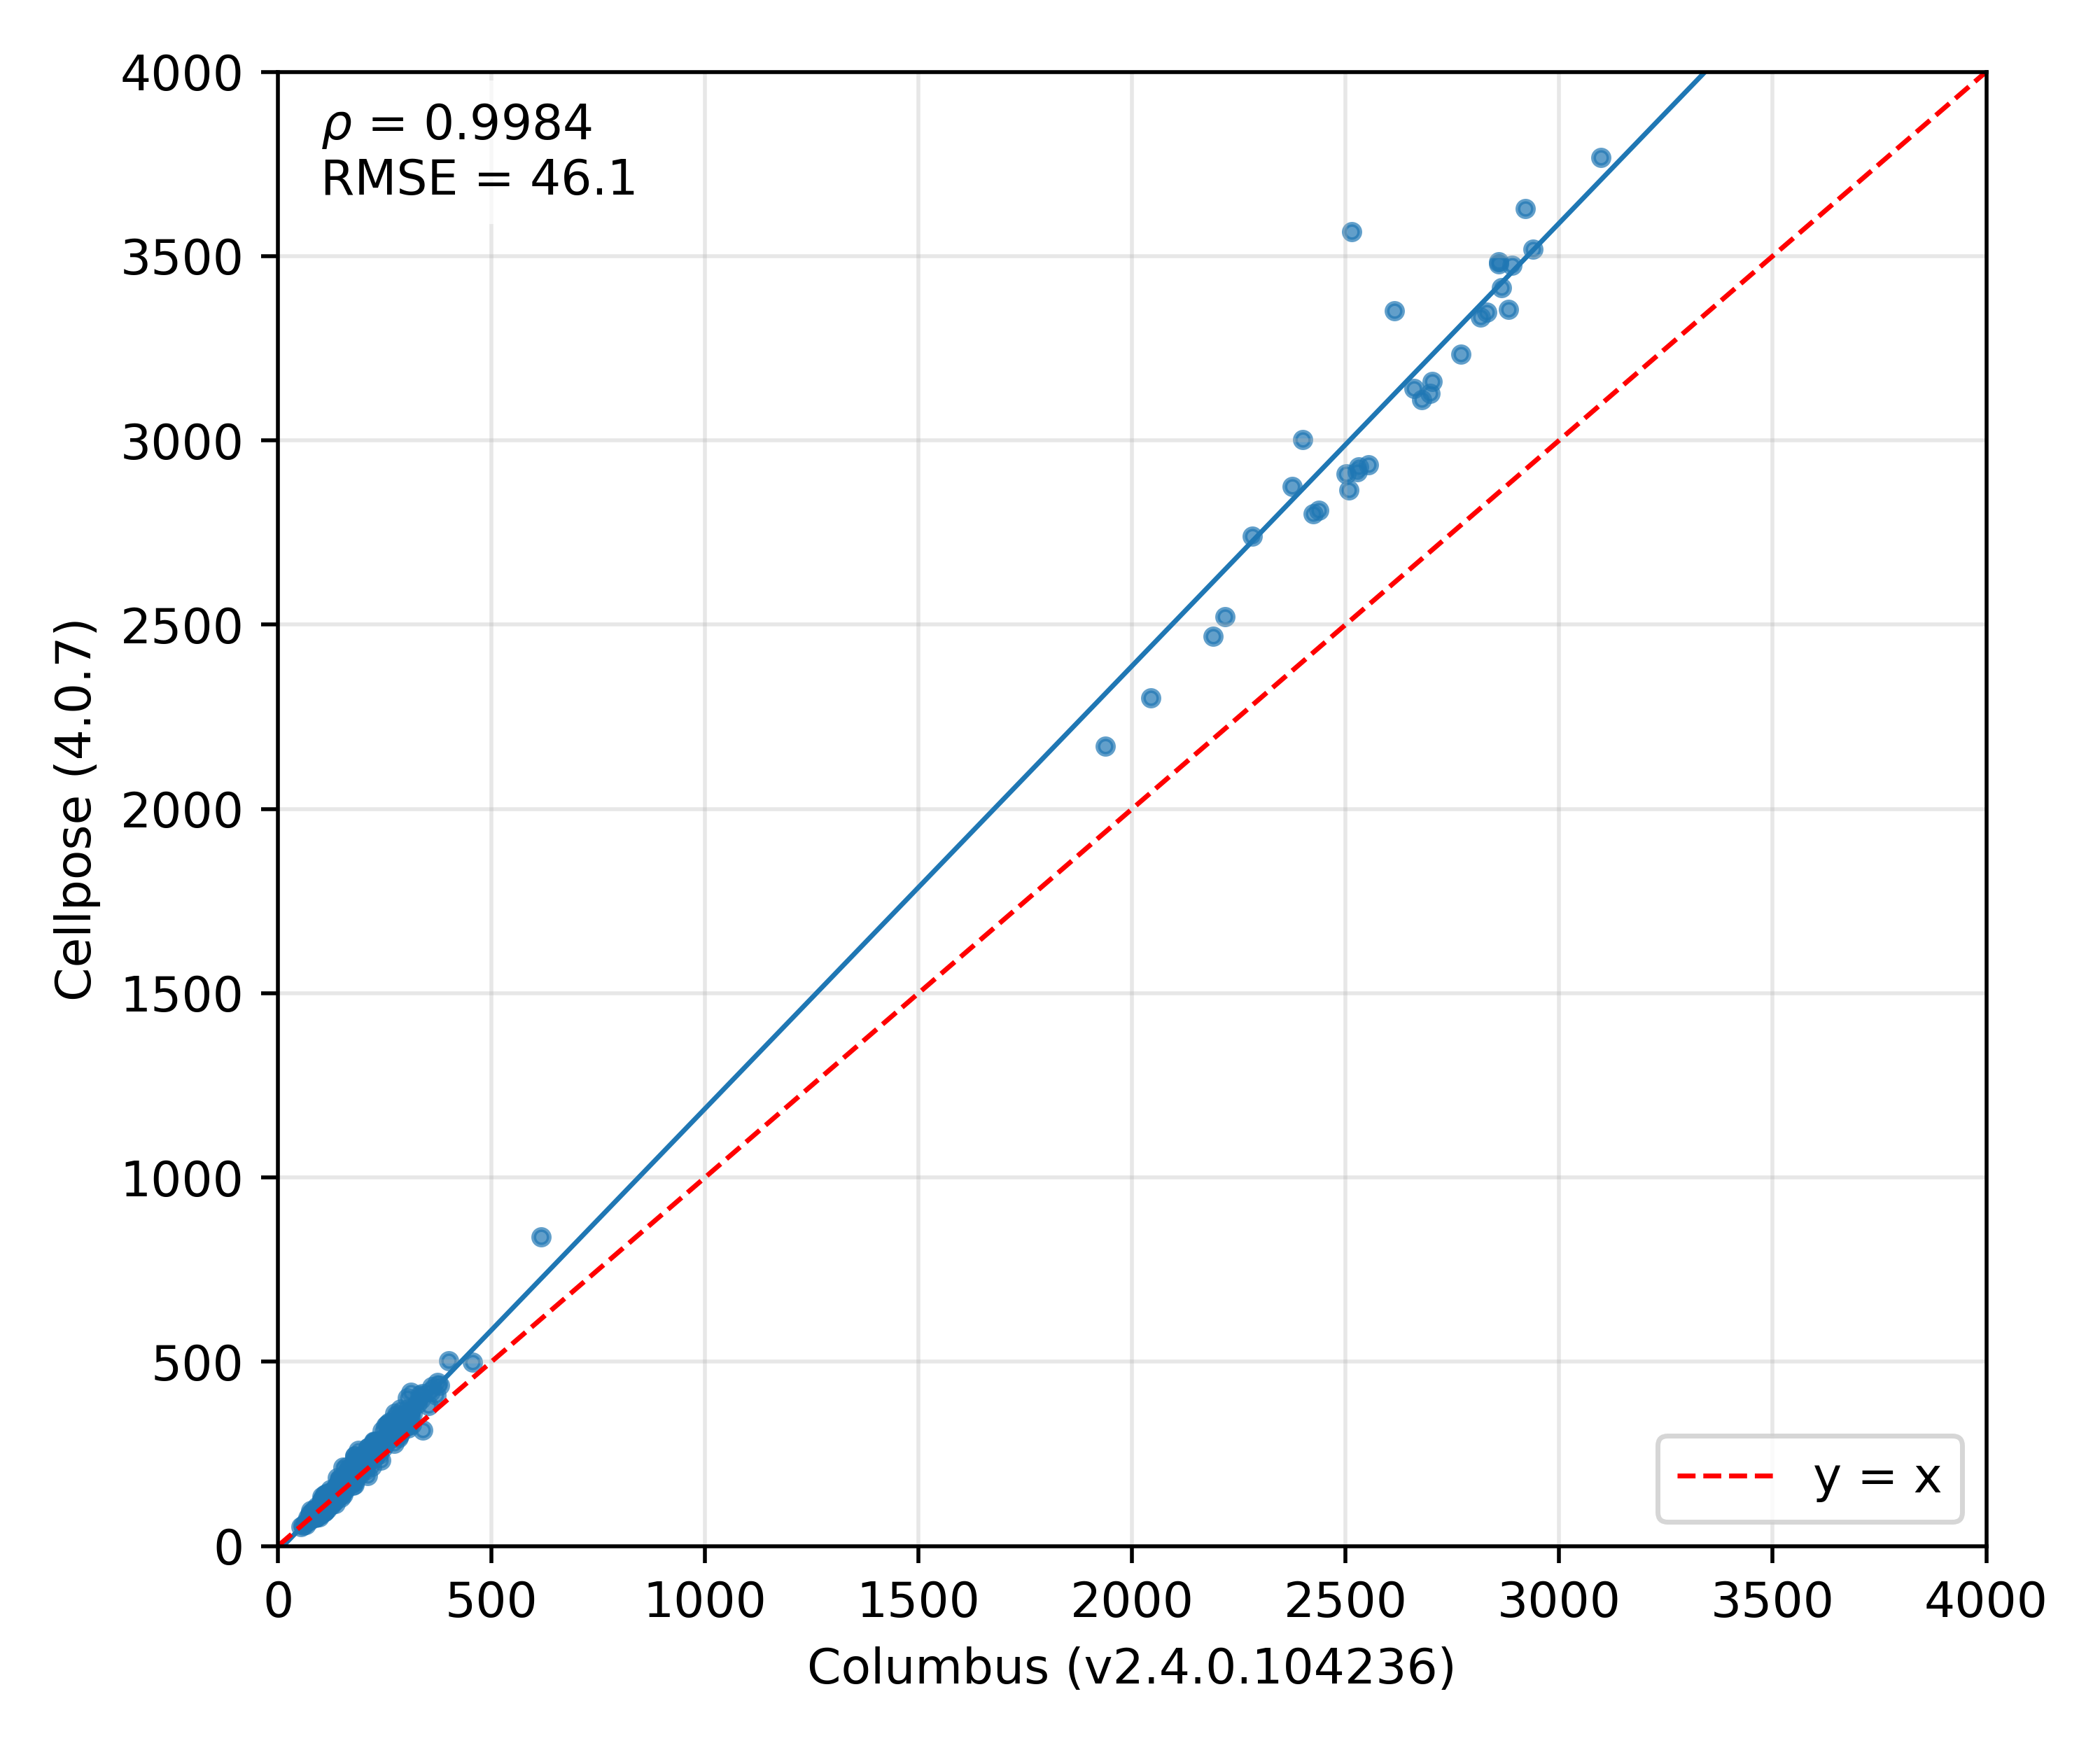
\includegraphics[width=\textwidth]{dispersion/Cellpose_4.0.7.png}
    \caption*{(B) Cellpose 4.0.7}
    \label{fig:cellpose407}
  \end{subfigure}
  \hfill
  \begin{subfigure}[b]{0.325\textwidth}
    \centering
    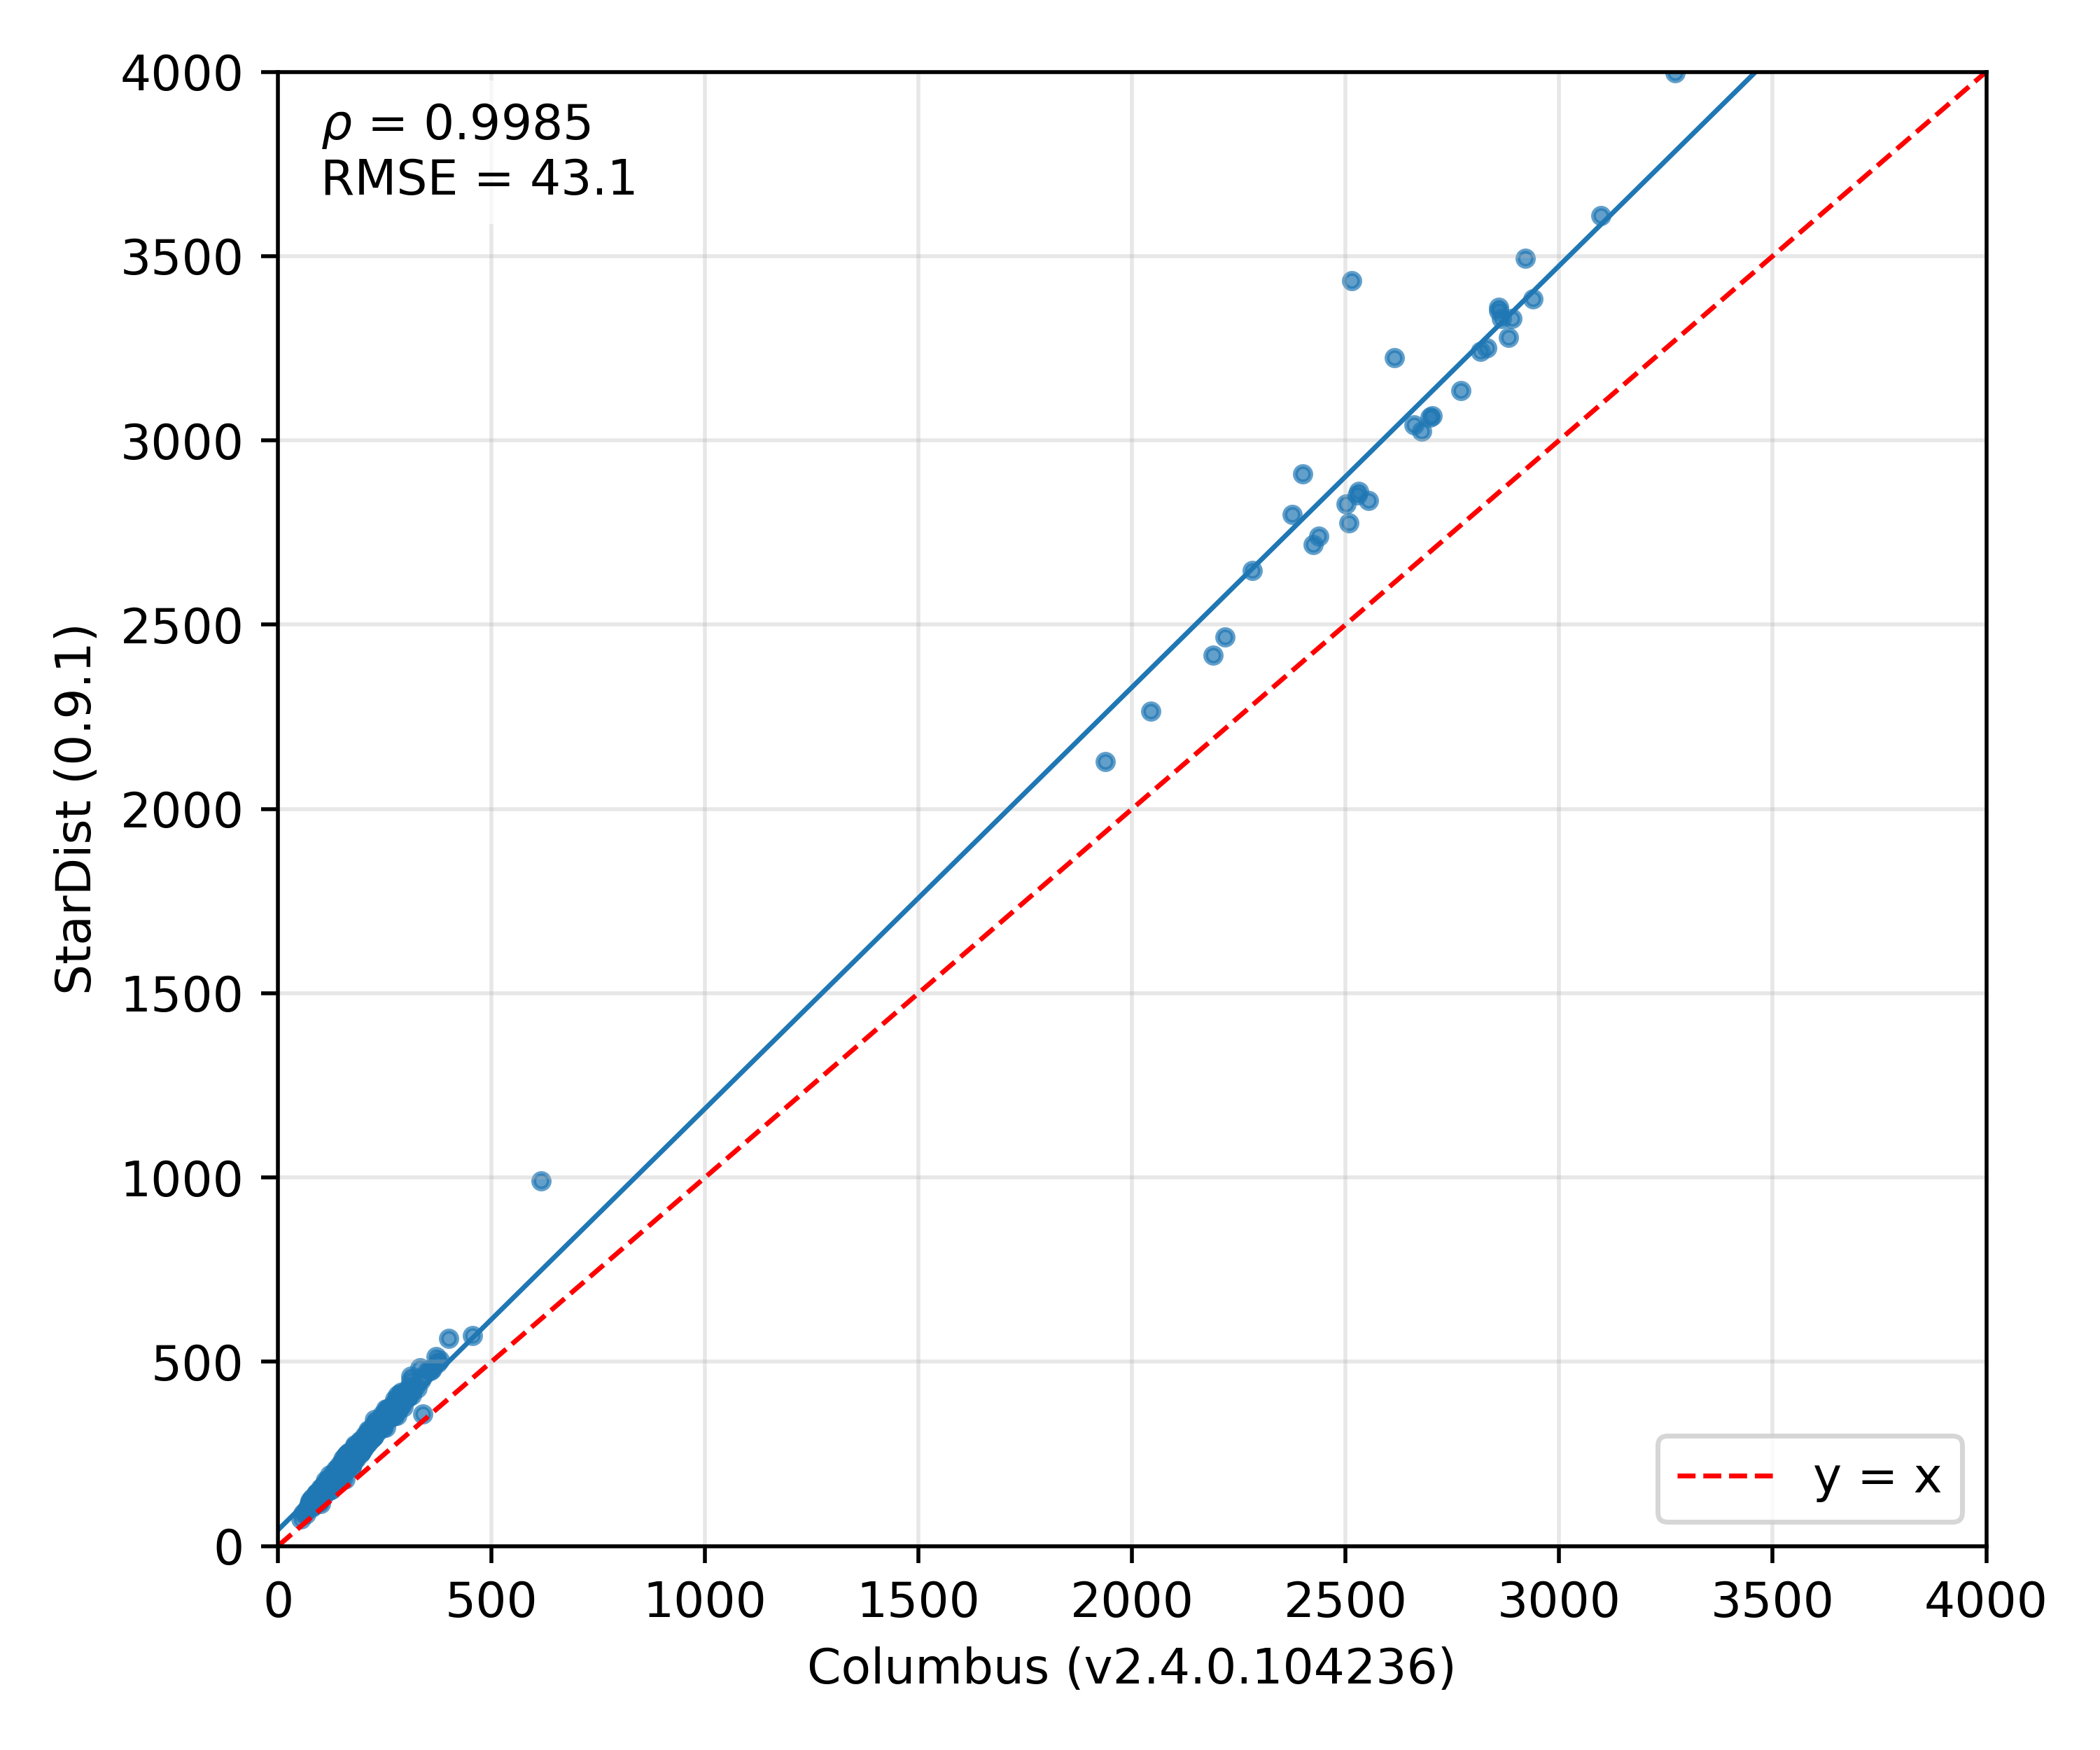
\includegraphics[width=\textwidth]{dispersion/StarDist_0.9.1.png}
    \caption*{(C) StarDist 0.9.1}
    \label{fig:stardist091}
  \end{subfigure}
  \caption{\textbf{Comparação entre as contagens de núcleos dos modelos avaliados e o método de referência.} O eixo X representa a contagem obtida pelo Acapella/Columbus, enquanto o eixo Y mostra as contagens dos modelos avaliados.}
  \label{fig:dispersion}
\end{figure}

A Figura \ref{fig:dispersion} apresenta a contagem de núcleos obtida por cada modelo avaliado em comparação com o método de referência. Todos os modelos apresentaram alta correlação com o software Acapella/Columbus, com $\rho \ge 0.9984$. A raiz do erro quadrático médio (do inglês, \textit{root mean square error}; RMSE) também foi calculada, indicando baixa divergência entre as contagens dos modelos avaliados e a referência. Esses resultados demonstram que os modelos avaliados são adequados para a tarefa de segmentação neste protocolo, oferecendo desempenho compatível com a solução comercial, com a vantagem adicional de serem ferramentas de código aberto. Apresentando apenas uma contagem ligeiramente superior ao método de referência em contextos de alta densidade celular.

A qualidade das segmentações foi avaliada visualmente, inspecionando as marcações dos núcleos sobrepostas às imagens originais (Figura \ref{fig:segmentation}).
Todos os modelos apresentaram boa qualidade de segmentação, com destaque para o StarDist 0.9.1, que demonstrou maior precisão na delimitação dos contornos dos núcleos, especialmente em regiões com alta densidade celular e sobreposição de núcleos. Os três modelos de código aberto superaram o método de referência em termos de qualidade visual das segmentações, onde podemos observar que o Columbus tende a subestimar a contagem de células em poços com alta densidade celular, possivelmente devido à dificuldade em segmentar núcleos sobrepostos, com diferenças de intensidade de fluorescência.

\begin{figure}[H]
  \centering
  \setlength{\tabcolsep}{6pt}
    % File information
    % >>> files[0] A01
    % '001001-1-001001001.tif'
    % >>> files[22] A23
    % '001023-1-001001001.tif'
    % >>> files[162] G19
    % '007019-1-001001001.tif'

    \begin{tabular}{>{\centering\arraybackslash}m{3.5cm} c c c}
      \toprule
      & \textbf{A01}
      & \textbf{G19}
      & \textbf{A23} \\
      & \scriptsize\textit{Controle negativo}
      & \scriptsize\textit{Caso experimental}
      & \scriptsize\textit{Controle positivo} \\
      \midrule

      % Row 1: Imagem bruta
      \footnotesize\textbf{Imagem bruta} &
      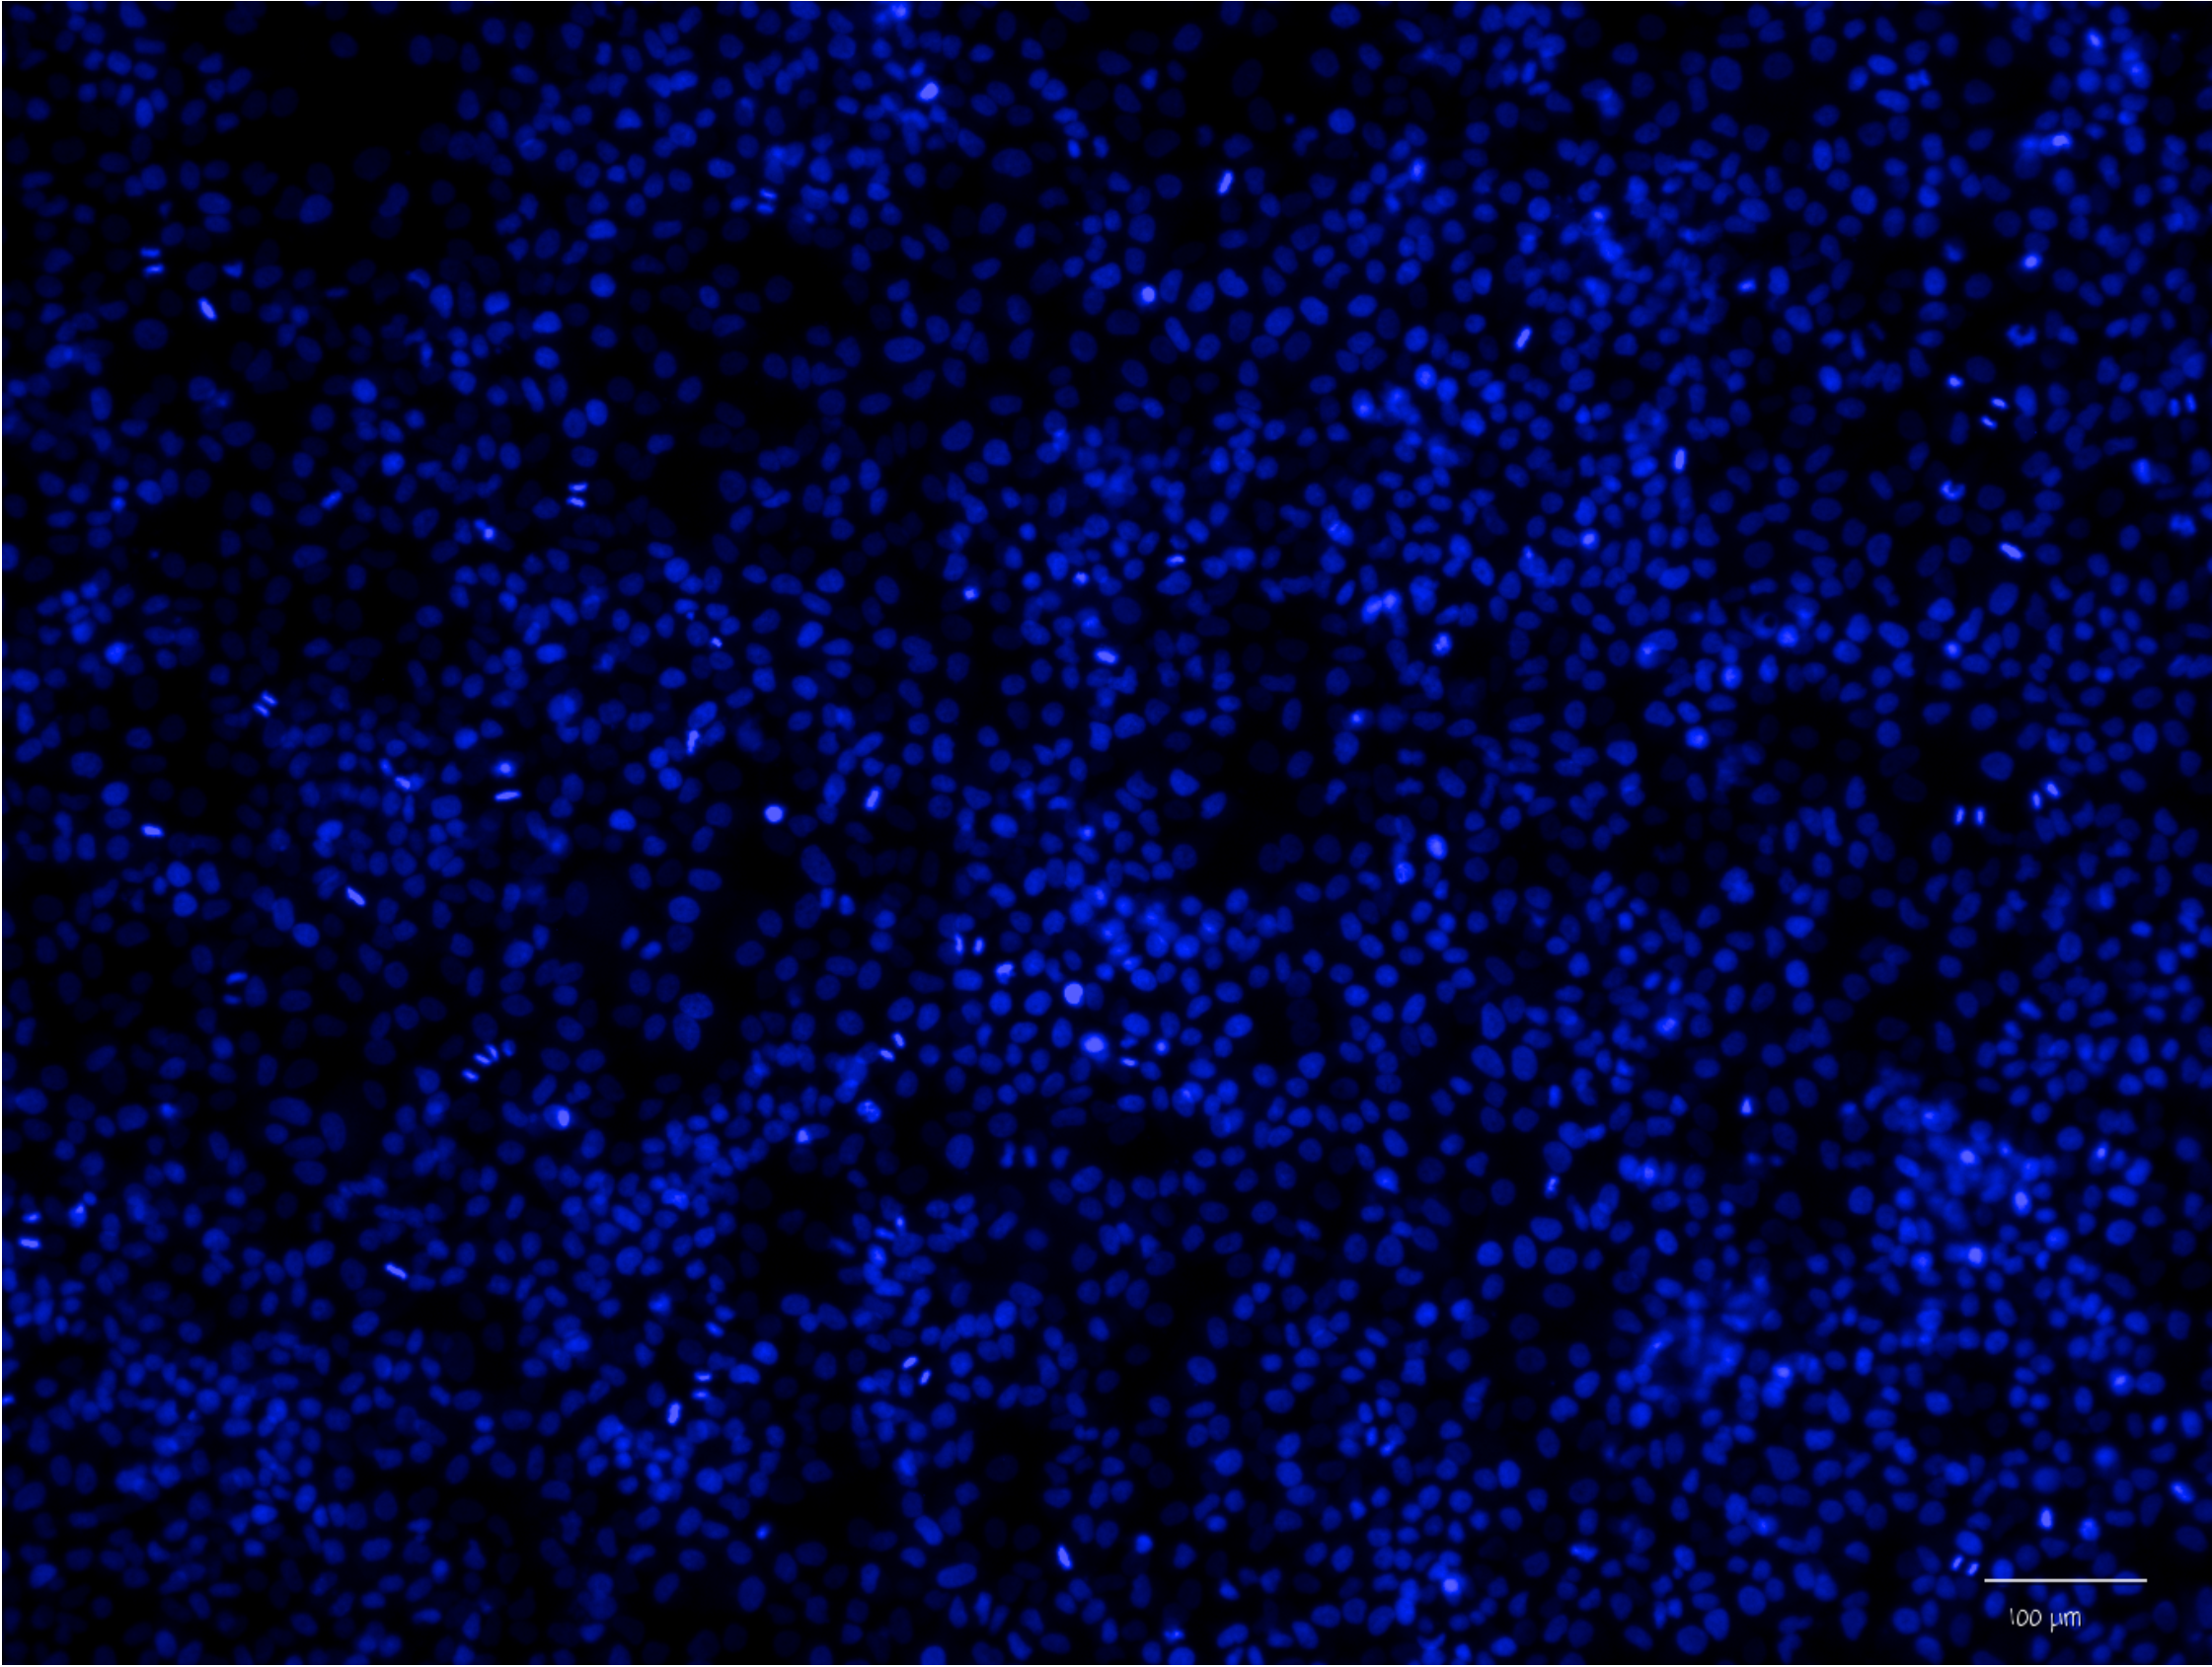
\includegraphics[width=0.23\textwidth, valign=m]{panel/A01.png} &
      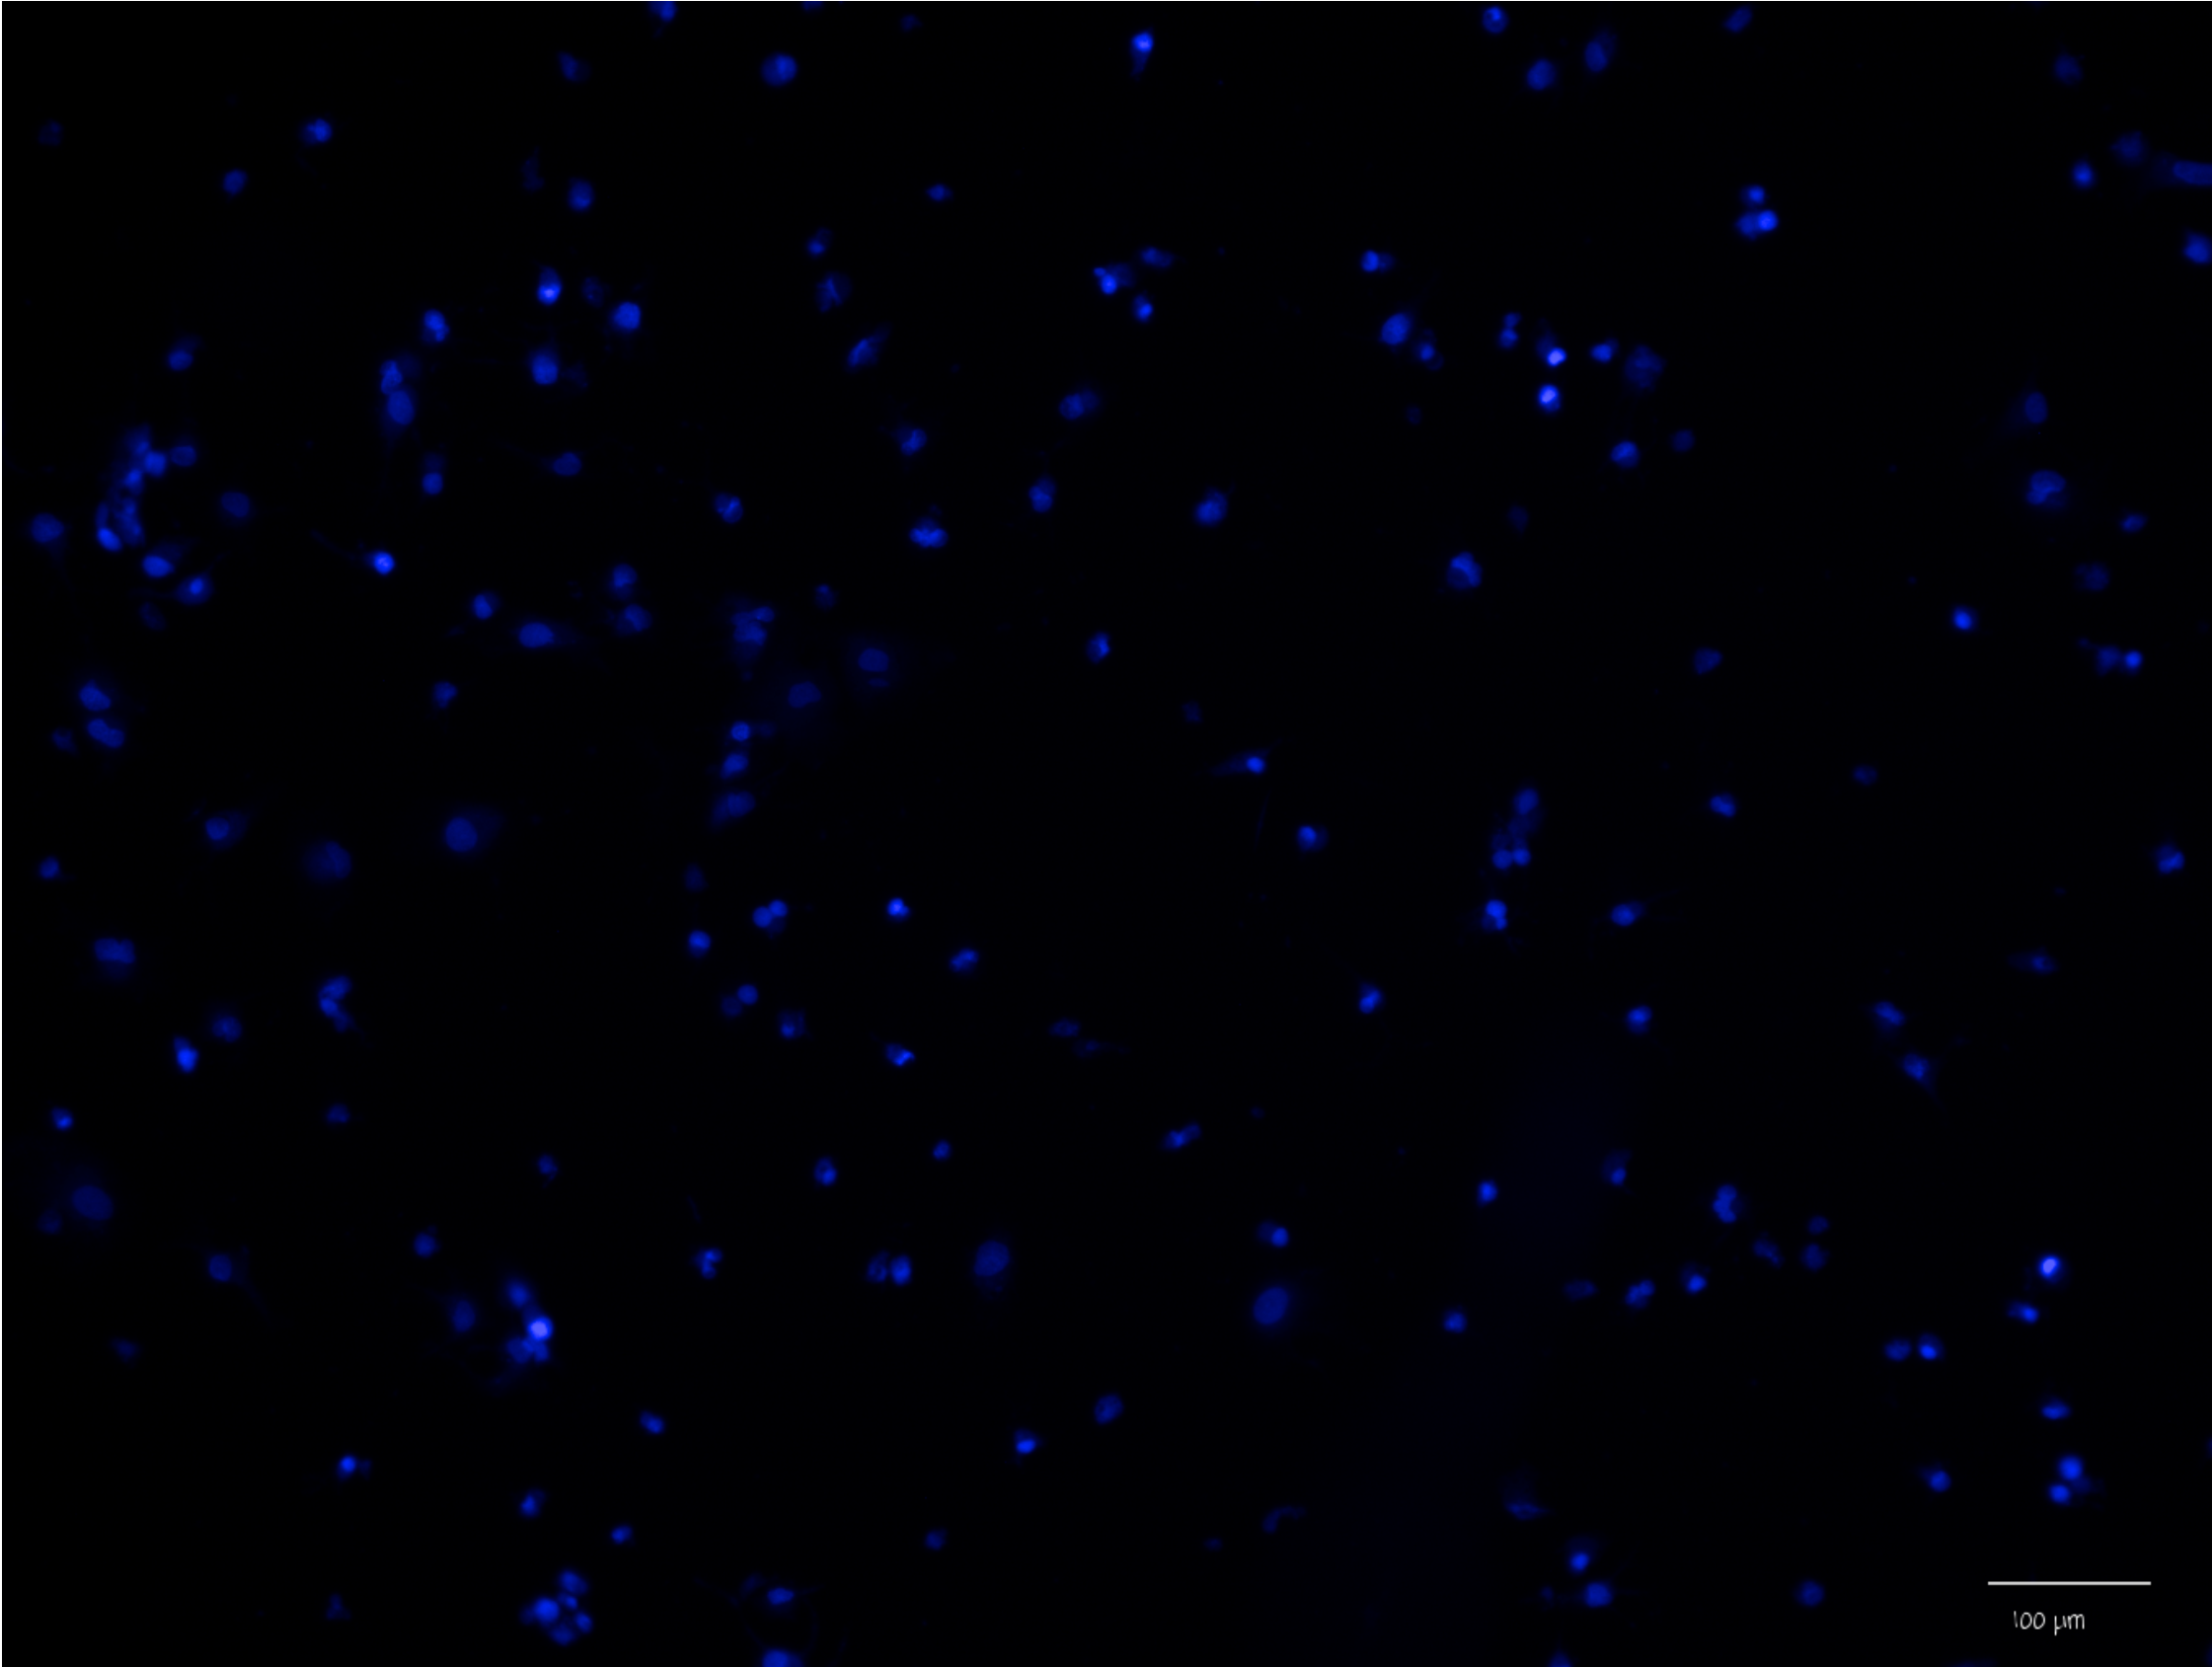
\includegraphics[width=0.23\textwidth, valign=m]{panel/G19.png} &
      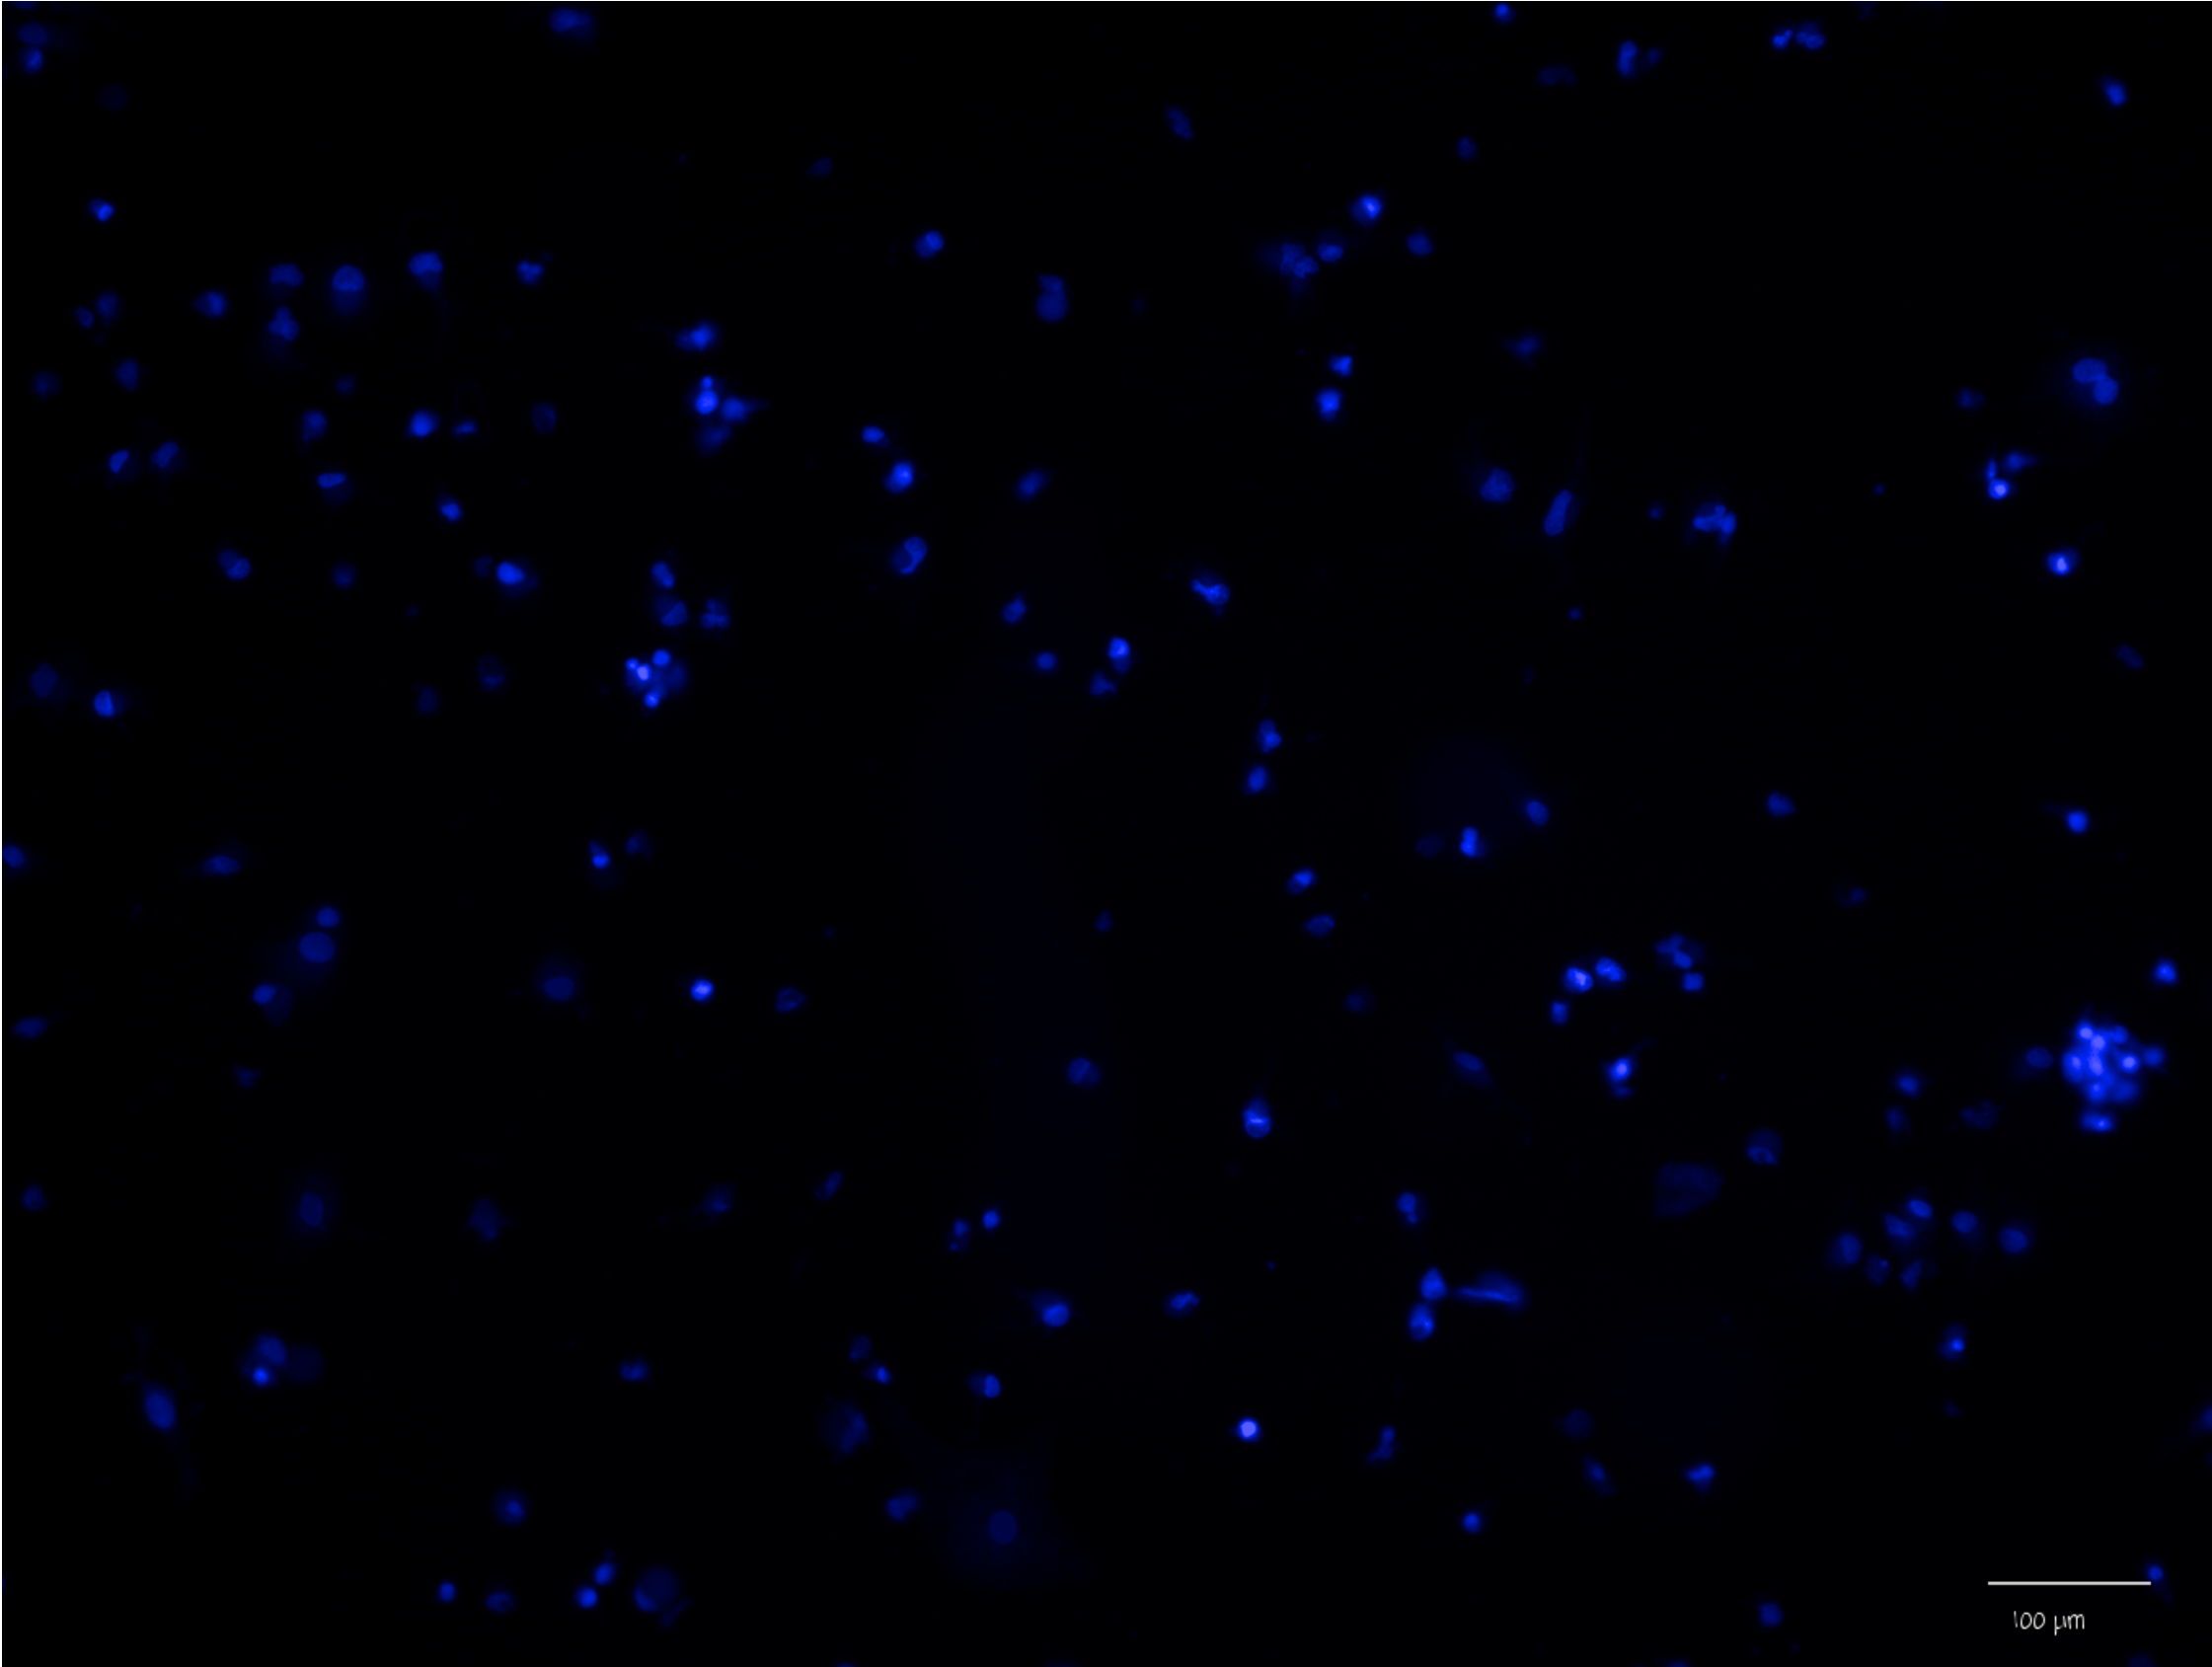
\includegraphics[width=0.23\textwidth, valign=m]{panel/A23.png} \\
      \specialrule{0.25pt}{2pt}{2pt}

      % Row 2: Columbus
      \footnotesize\textbf{Columbus (v2.4.0.104236)} &
      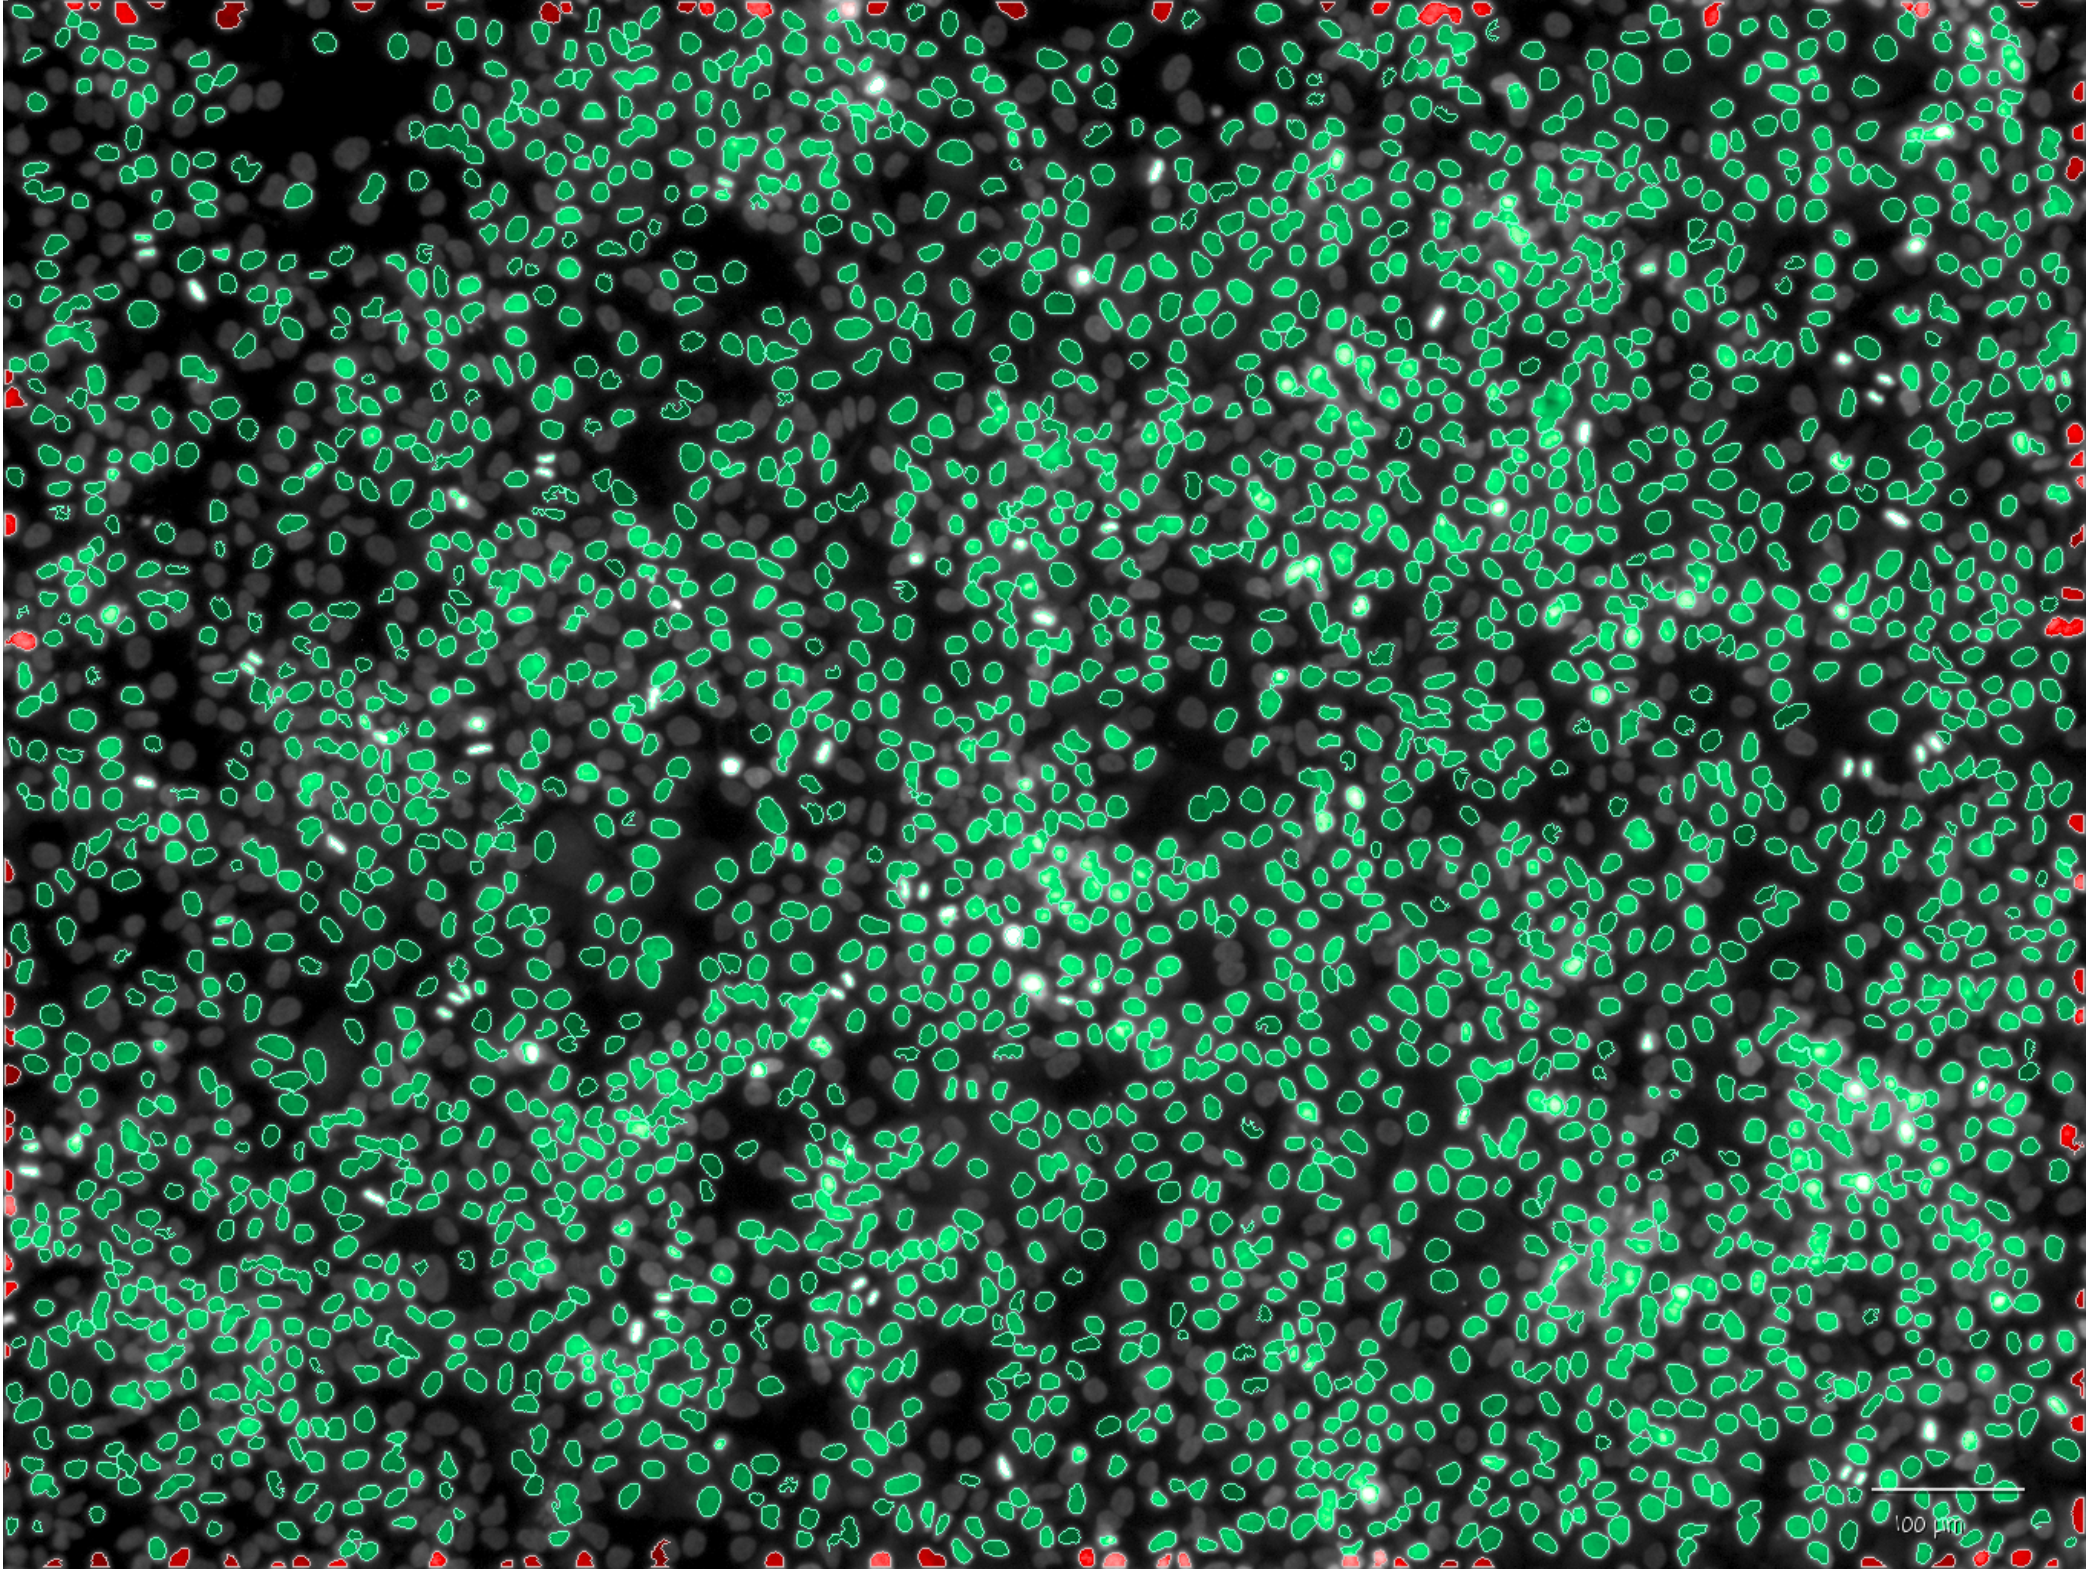
\includegraphics[width=0.23\textwidth, valign=m]{panel/columbus_SLEV_S1_A01.png} &
      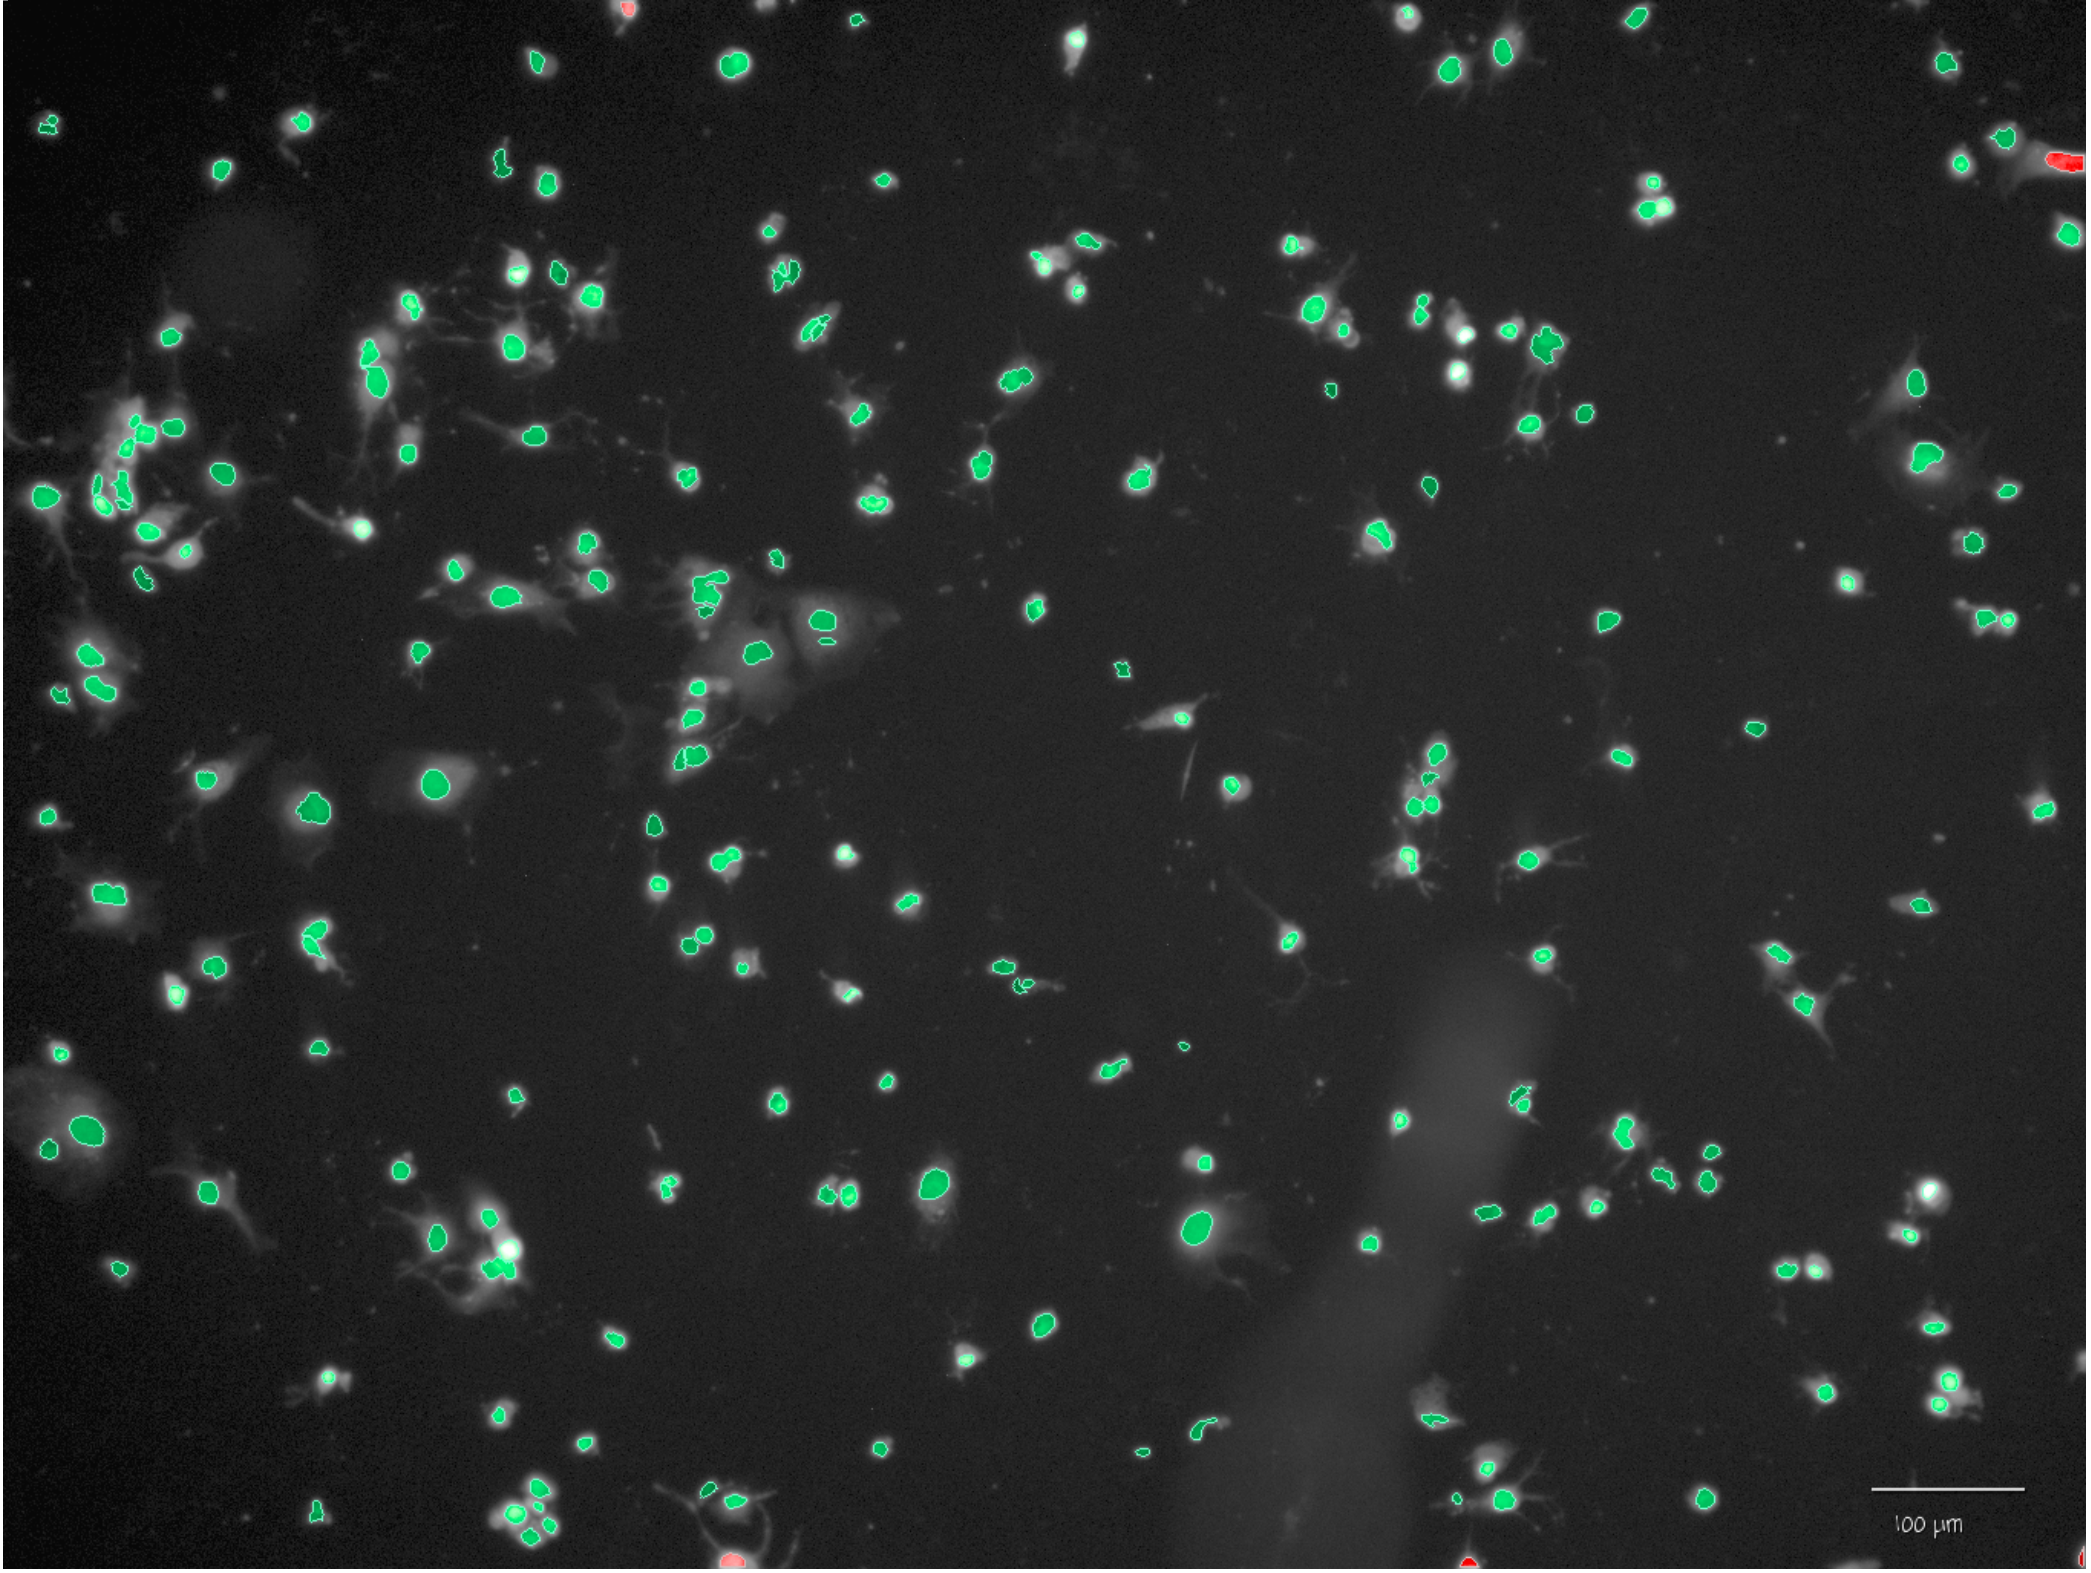
\includegraphics[width=0.23\textwidth, valign=m]{panel/columbus_SLEV_S1_G19.png} &
      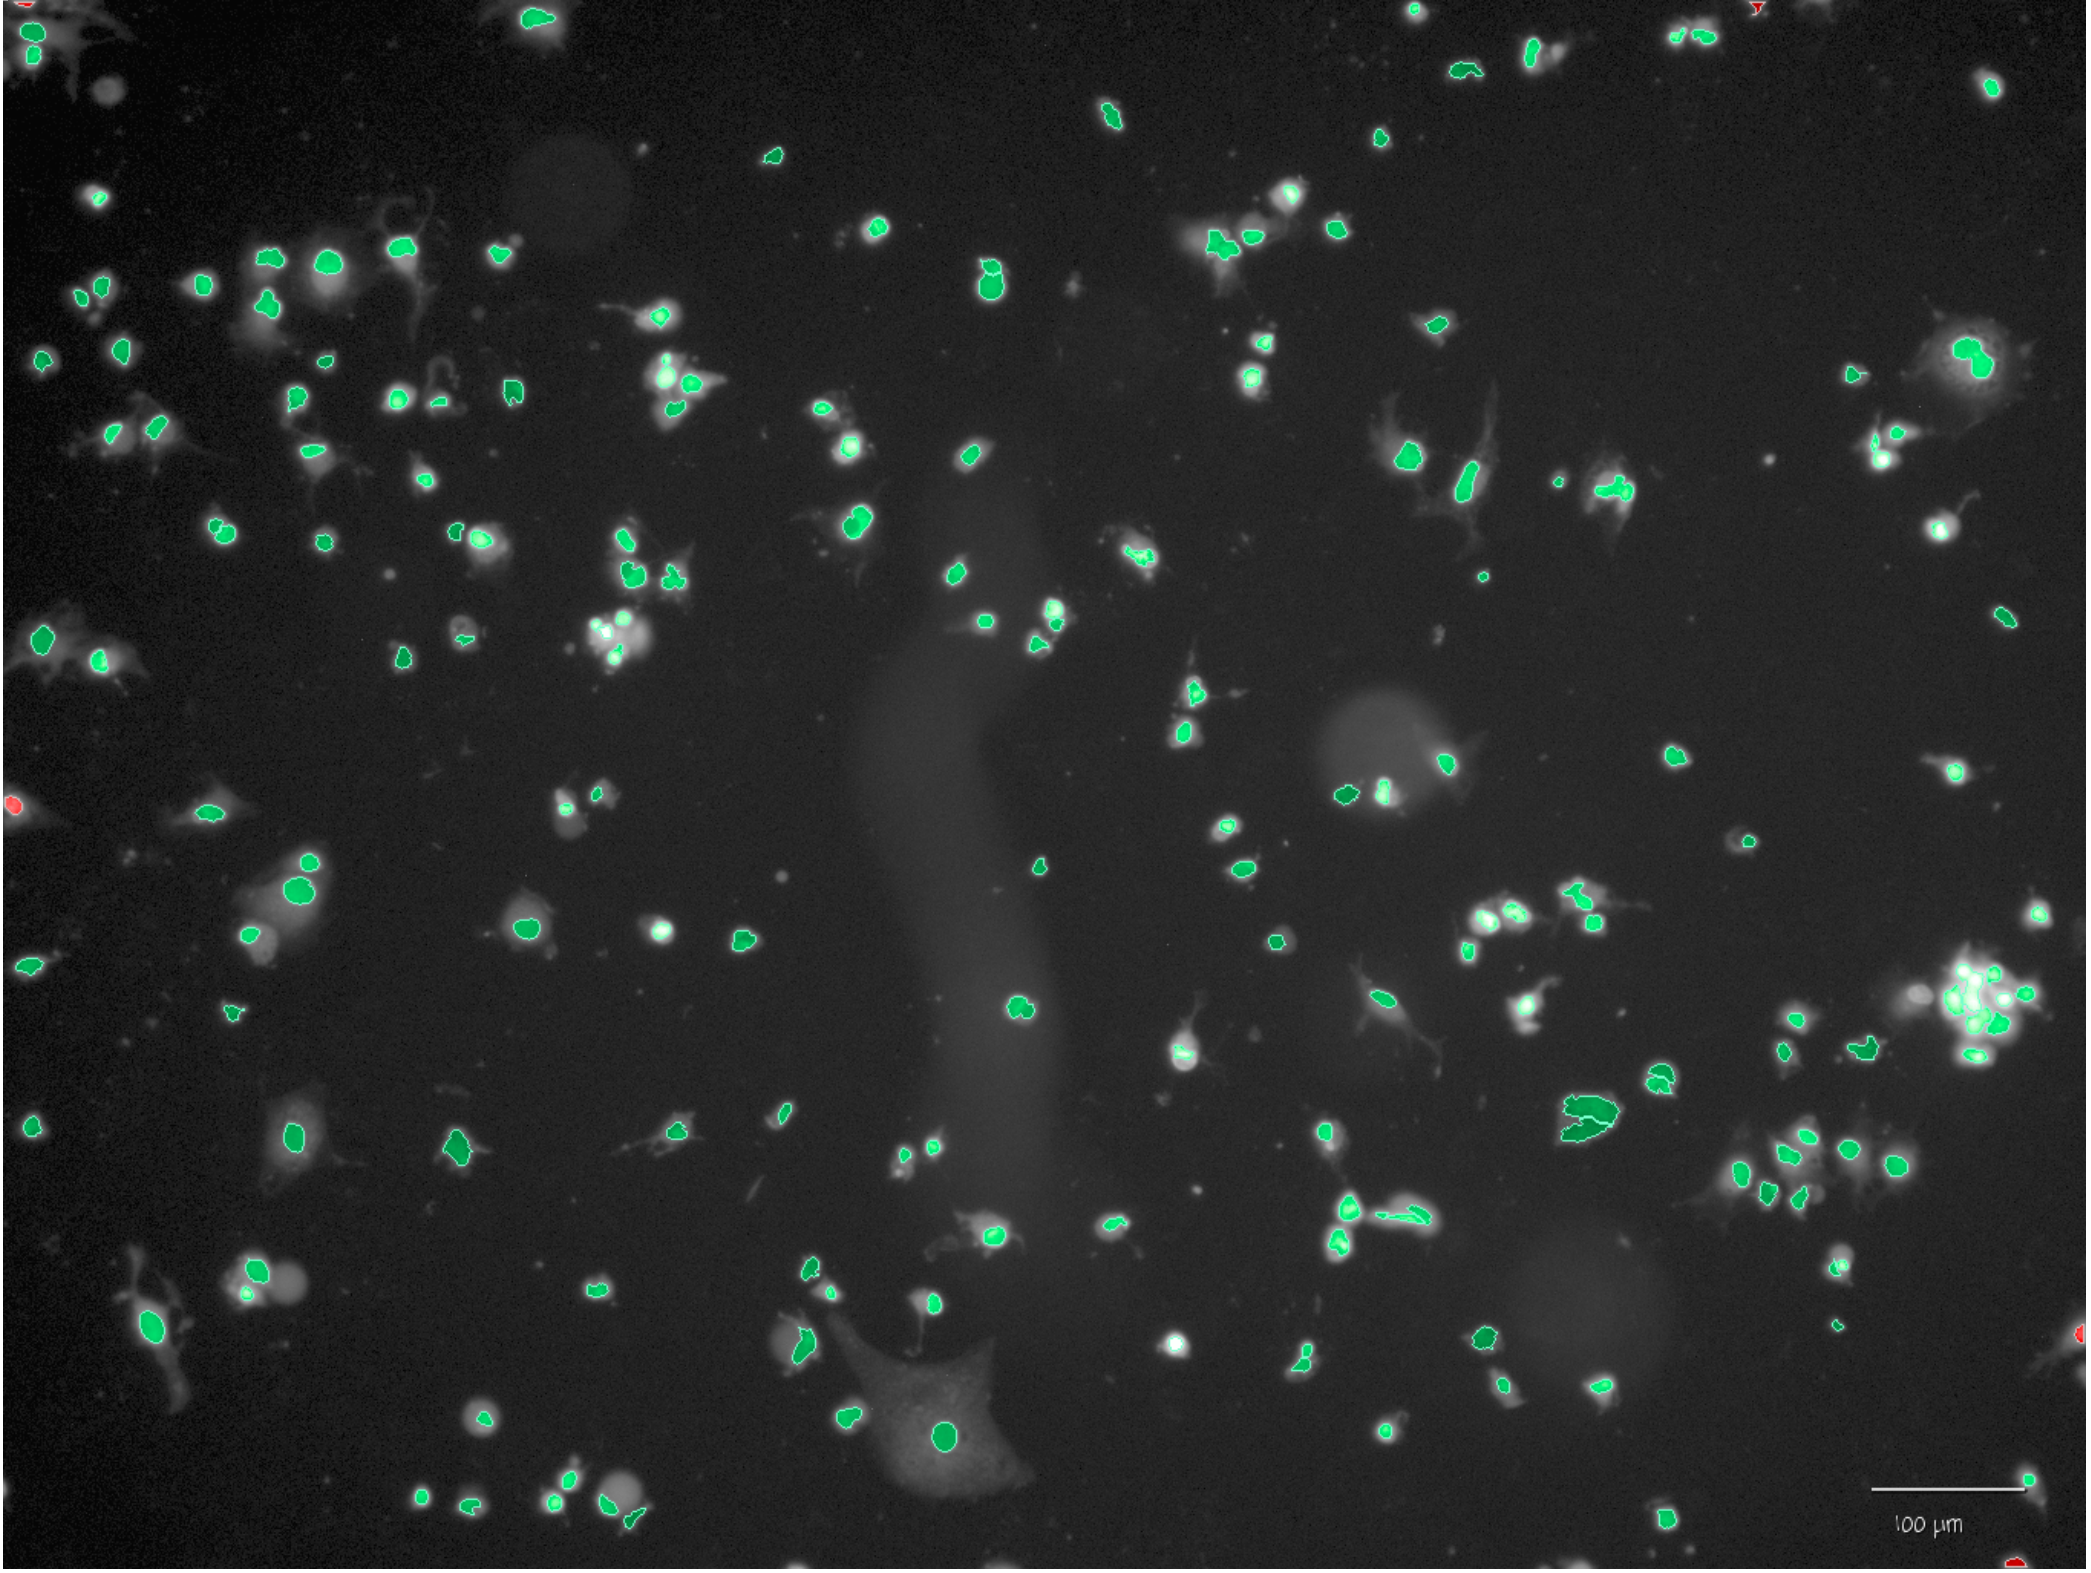
\includegraphics[width=0.23\textwidth, valign=m]{panel/columbus_SLEV_S1_A23.png} \\
      &
      \scriptsize$N_c = 2515$ &
      \scriptsize$N_c = 204$ &
      \scriptsize$N_c = 184$ \\
      \specialrule{0.25pt}{2pt}{2pt}

      % Row 3: Cellpose 3.1.1.2
      \footnotesize\textbf{Cellpose (v3.1.1.2)} &
      
\includegraphics[width=0.23\textwidth, valign=m]{panel/cellpose3_SLEV_S1_A01.png} &
      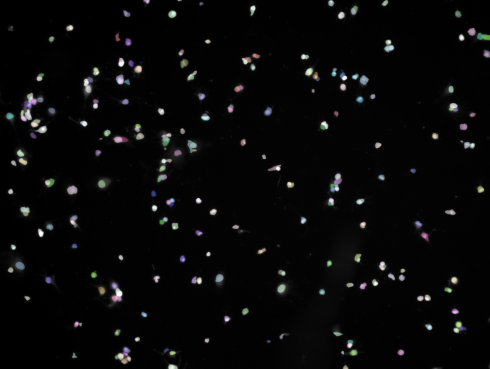
\includegraphics[width=0.23\textwidth, valign=m]{panel/cellpose3_SLEV_S1_G19.png} &
      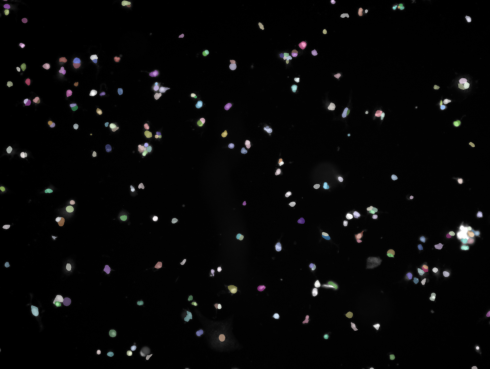
\includegraphics[width=0.23\textwidth, valign=m]{panel/cellpose3_SLEV_S1_A23.png} \\
      &
      \scriptsize$N_c = 3483$ &
      \scriptsize$N_c = 249$ &
      \scriptsize$N_c = 221$ \\
      \specialrule{0.25pt}{2pt}{2pt}

      % Row 4: Cellpose 4.0.7
      \footnotesize\textbf{Cellpose (v4.0.7)} &
      
\includegraphics[width=0.23\textwidth, valign=m]{panel/cellpose4_SLEV_S1_A01.png} &
      
\includegraphics[width=0.23\textwidth, valign=m]{panel/cellpose4_SLEV_S1_G19.png} &
      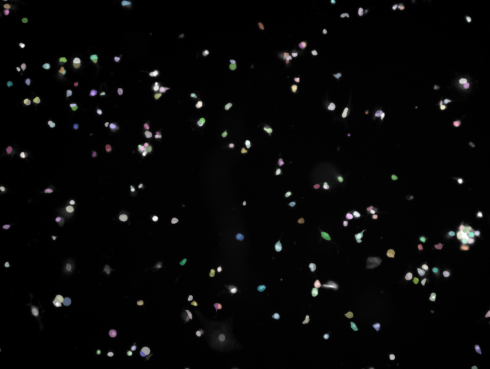
\includegraphics[width=0.23\textwidth, valign=m]{panel/cellpose4_SLEV_S1_A23.png} \\
      &
      \scriptsize$N_c = 3566$ &
      \scriptsize$N_c = 228$ &
      \scriptsize$N_c = 189$ \\
      \specialrule{0.25pt}{2pt}{2pt}

      % Row 5: StarDist 0.9.1
      \footnotesize\textbf{StarDist (v0.9.1)} &
      
\includegraphics[width=0.23\textwidth, valign=m]{panel/stardist_SLEV_S1_A01.png} &
      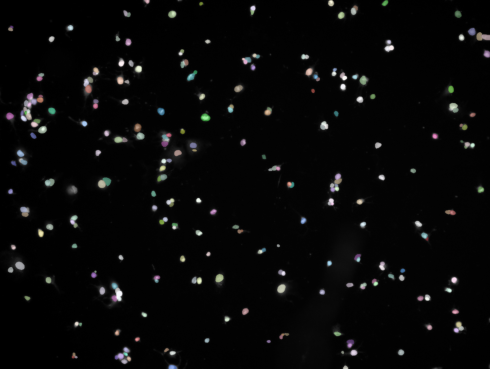
\includegraphics[width=0.23\textwidth, valign=m]{panel/stardist_SLEV_S1_G19.png} &
      
\includegraphics[width=0.23\textwidth, valign=m]{panel/stardist_SLEV_S1_A23.png} \\
      &
      \scriptsize$N_c = 3433$ &
      \scriptsize$N_c = 272$ &
      \scriptsize$N_c = 239$ \\

      \bottomrule
    \end{tabular}

  \caption{\textbf{Comparação visual de segmentações obtidas pelo software Columbus (v2.4).} Imagens brutas e segmentações para poços representativos: controle negativo (A01), caso experimental (G19) e controle positivo (A23).}
  \label{fig:segmentation}
\end{figure}

Do ponto de vista computacional, também avaliamos o tempo de processamento e o uso de memória de vRAM da GPU para cada modelo. A Figura \ref{fig:performance} apresenta o tempo médio de processamento por imagem e o uso de memória de vRAM da GPU para apenas cada modelo avaliado.

\begin{figure}[ht]
\centering

  \begin{tikzpicture}
    \begin{axis}[
        ybar,
        bar width=20pt,
        width=0.49\textwidth,
        height=0.475\textwidth,
        ymin=0,
        ylabel={Tempo $\left(\frac{s}{\texttt{imagem}}\right)$},
        symbolic x coords={
            Cellpose (3.1.1.2),
            Cellpose (4.0.7),
            StarDist (0.9.1)
        },
        xtick=data,
        xticklabel style={align=center, rotate=0, font=\tiny},
        enlarge x limits=0.25,
    ]
    \addplot+[
        error bars/.cd,
            y dir=both,
            y explicit,
    ] coordinates {
        (Cellpose (3.1.1.2), 4.013020833) +- (0, 0.028645833)
        (Cellpose (4.0.7),   2.213541667) +- (0,  0.0078125)
        (StarDist (0.9.1),   0.690104167) +- (0,  0.005208333)
    };
    \end{axis}
  \end{tikzpicture}
  \hfill
  \begin{tikzpicture}
    \begin{axis}[
        ybar,
        bar width=20pt,
        width=0.49\textwidth,
        height=0.475\textwidth,
        ymin=0,
        ylabel={Memória vRAM (GB)},
        symbolic x coords={
            Cellpose (3.1.1.2),
            Cellpose (4.0.7),
            StarDist (0.9.1)
        },
        xtick=data,
        xticklabel style={align=center, rotate=0, font=\tiny},
        enlarge x limits=0.25,
    ]
    \addplot coordinates {
        (Cellpose (3.1.1.2), 0.2)
        (Cellpose (4.0.7),   1.9)
        (StarDist (0.9.1),   6.2)
    };
    \end{axis}
  \end{tikzpicture}

  \caption{\textbf{Desempenho computacional dos métodos de segmentação.} (A) Tempo médio de processamento por imagem. (B) Uso médio de memória vRAM da GPU. Os experimentos foram executados no servidor de desenvolvimento com 48 GPUsuma GPU NVIDIA A100 (40~GB vRAM). Barras de erro indicam o desvio padrão.}
  \label{fig:performance}
\end{figure}

Levando em conta o desempenho computacional e a qualidade das segmentações, o modelo StarDist 0.9.1 foi selecionado para implementação no protocolo final de processamento de imagens do pacote \texttt{CellViability}. Esse modelo apresentou o melhor equilíbrio entre precisão na segmentação e eficiência computacional, sendo capaz de processar as imagens em um tempo razoável, mesmo com um uso mais elevado de memória vRAM da GPU. Pensando em maturidade do software, ele ainda está em fase beta de desenvolvimento, como indicado em sua versão mais recente (v0.9.1). No entanto, sua performance superior na segmentação de núcleos celulares justifica sua escolha para o protocolo, garantindo resultados confiáveis e de alta qualidade para a análise fenotípica de viabilidade celular. Porém, o protocolo foi estruturado de forma modular, permitindo a fácil substituição do modelo de segmentação no futuro, caso novas versões ou modelos alternativos apresentem melhorias significativas.

\subsubsection{Extração de características morfológicas}

A partir das segmentações, as características morfológicas dos núcleos foram extraídas com scikit-image \cite{vanderWalt2014}, incluindo área, perímetro e excentricidade, que são apresentadas ao usuário como uma planilha de Excel, nomeada \texttt{morphology.xlsx}, por placa. Além disso, foi calculada a contagem total de células por poço, que servirá como métrica primária para avaliar a viabilidade celular nos ensaios.

\subsubsection{Normalização dos dados}

A partir da contagem total de cada poço, a inibição do efeito citopático (inCPE) viral foi calculada, conforme a equação a seguir:

\begin{equation}
  \mathrm{inCPE} = \frac{N_{c} - \mu_{c^{+}}}{\mu _{c^{-}} - \mu_{c^{+}}}
\end{equation}

\noindent onde $N_{c}$ é a contagem de núcleos no poço avaliado, $\mu _{c^{+}}$ é a média das contagens dos controles positivos (infectados, sem tratamento) e $\mu _{c^{-}}$ é a média das contagens dos controles negativos (não infectados, sem tratamento) da mesma placa.

Essa normalização reduz o impacto de variações sistemáticas entre placas e facilita comparações diretas entre condições experimentais.

\subsubsection{Controle de qualidade das placas}

A qualidade das placas de ensaios de viabilidade celular foi avaliada pelo Z'-factor ($Z'$) \cite{Zhang,Zhang1999}, um índice estatístico que avalia a variabilidade dos dados entre os controles positivo (infectado e não tratado) e negativo (não infectado e não tratado). O $Z'$ é calculado conforme a equação:

\begin{equation}
  Z^\prime = 1 - \frac{3\sigma_{c^{+}} + 3\sigma_{c^{-}}}{\left|\mu_{c^{+}} - \mu_{c^{-}}\right|},
\end{equation}

onde $\sigma _{c^{+}}$ e $\sigma _{c^{-}}$ representam os desvios padrão dos controles positivo e negativo, respectivamente, e $\mu _{c^{+}}$ e $\mu _{c^{-}}$ correspondem às suas médias.

Conforme estabelecido na literatura \cite{Zhang1999,Bray2004}, os valores de $Z'$ são interpretados da seguinte forma:

\begin{itemize}
  \item $Z' = 1,0$: ensaio ideal, com separação perfeita entre os controles positivo e negativo;
  \item $0,5 < Z' \leq 1,0$: ensaio de alta qualidade, com boa separação entre os controles positivo e negativo;
  \item $0 < Z' \leq 0,5$: ensaio aceitável, mas com alguma sobreposição entre os controles;
  \item $Z' = 0$: ensaio sem separação entre os controles positivo e negativo;
  \item $Z' < 0$: ensaio de baixa qualidade, com significativa sobreposição entre os controles.
\end{itemize}

Com base nessas interpretações, as placas com $Z'$ menores que um limiar definido pelo usuário (por padrão, $Z' < 0,5$) serão excluídas das análises subsequentes. Um arquivo nomeado \texttt{status}, é gerado no diretório de saída de cada placa, contendo \texttt{SUCCESS} ou \texttt{FAILED}, indicando se a placa foi aprovada ou reprovada no controle de qualidade, respectivamente.

Para a placa S1 do ensaio de viabilidade celular contra o vírus SLEV, o valor calculado foi $Z' = 0.43$. Considerando o limiar para ensaio de alta qualidade ($0,5 < Z' \leq 1,0$), essa placa não foi aprovada no controle de qualidade e, portanto, não foi incluída na seleção dos compostos candidatos (\textit{hits}). Porém, adotando um critério menos rigoroso, considerando placas aceitáveis ($0 < Z' \leq 0,5$), a placa S1 poderia ser incluída na análise.

\subsubsection{Visualização dos dados}

A visualização dos resultados foi realizada utilizando as bibliotecas matplotlib (Hunter, 2007) e Plotly. As marcações dos núcleos segmentados são sobrepostas às imagens originais e salvas em formato PNG em uma estrutura de diretórios hierárquica definida pelo usuário. Especificamente, as imagens são armazenadas dentro de um diretório base informado via linha de comando (--basedir), seguido por subdiretórios correspondentes ao nome do screening (i.e., SLEV), ao identificador da placa (e.g., S1) e ao diretório instances (\eg, \texttt{results/SLEV/S1/instances/*.png}). Essas imagens facilitam a inspeção visual da qualidade da segmentação e a identificação de possíveis artefatos (Figura \ref{fig:segmentation}; StarDist (v0.9.1)). Essas imagens permitem a inspeção visual sistemática da qualidade da segmentação e a identificação de possíveis artefatos.

Os dados quantitativos derivados da análise, como a contagem de células ($N_c$) e o índice normalizado de efeito citopático (inCPE), são apresentados na forma de mapas de placa interativos em formato HTML (Figura \ref{fig:visualization}). Essas visualizações facilitam a interpretação dos resultados experimentais, permitindo a rápida identificação de padrões espaciais, efeitos de borda e variações associadas às diferentes condições experimentais.

\begin{figure}[ht]
  \centering
  \begin{subfigure}[b]{0.49\textwidth}
    \centering
    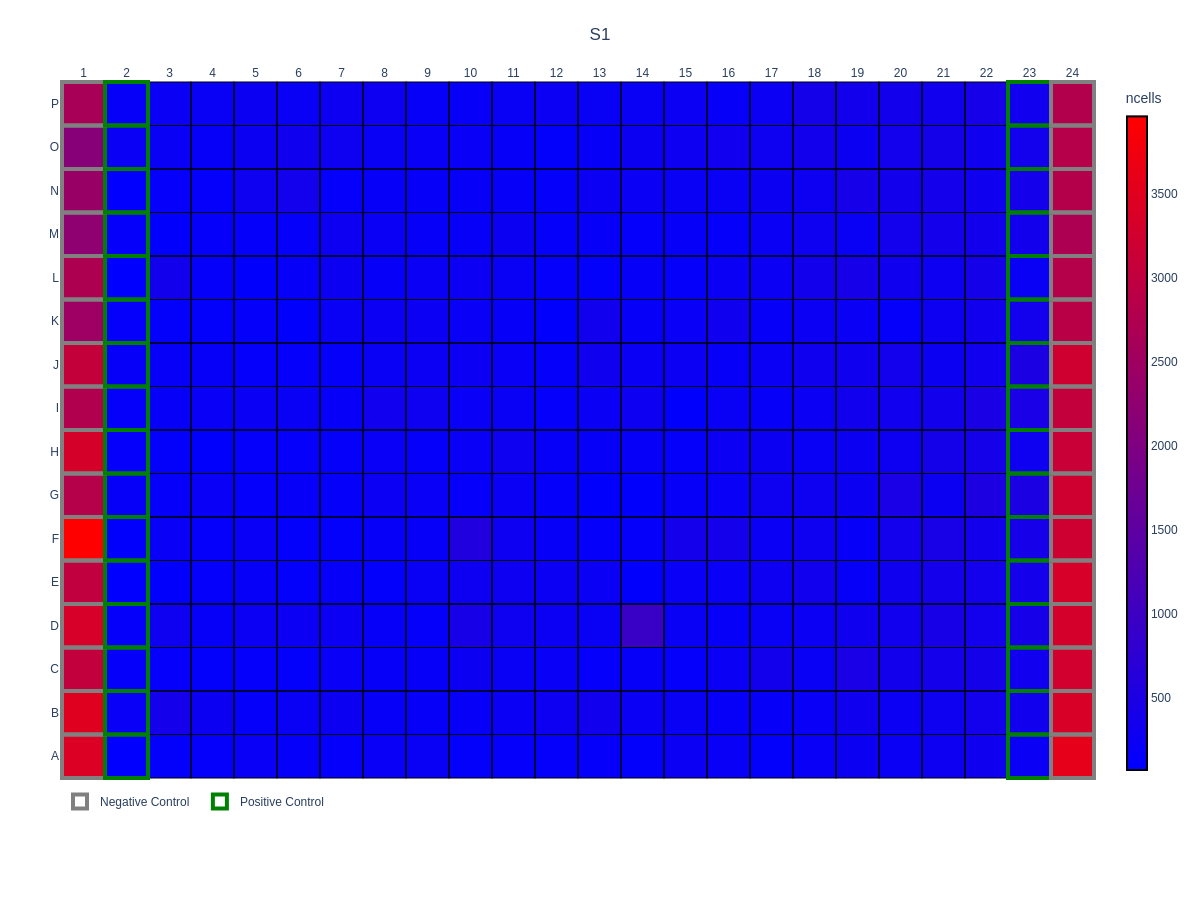
\includegraphics[width=\textwidth]{visualization/ncells.png}
    \caption*{(A) Contagem de células ($N_c$).}
    \label{fig:overlay}
  \end{subfigure}
  \hfill
  \begin{subfigure}[b]{0.49\textwidth}
    \centering
    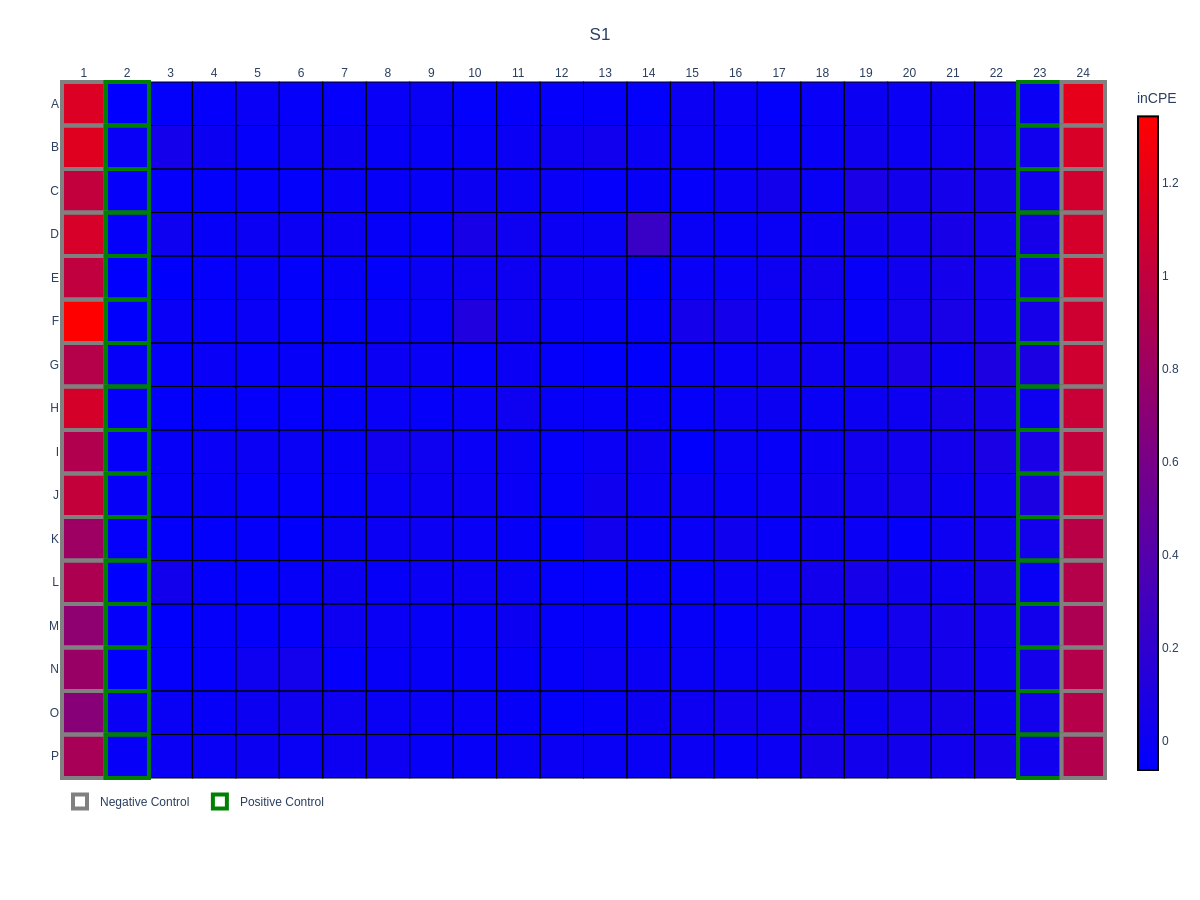
\includegraphics[width=\textwidth]{visualization/incpe.png}
    \caption*{(B) inCPE.}
    \label{fig:plate_map}
  \end{subfigure}
  \caption{\textbf{Exemplos de visualizações geradas pelo protocolo \texttt{CellViability}.} (A) Exemplo de sobreposição das segmentações dos núcleos sobre a imagem original para inspeção visual. (B) Exemplo de mapa interativo da placa, exibindo os valores de inCPE por poço.}
  \label{fig:visualization}
\end{figure}

\subsubsection{Integração dos dados e seleção dos compostos candidatos (\textit{hits})}

Após a aprovação das placas na etapa de controle de qualidade, os dados quantitativos extraídos das imagens foram integrados em nível de screening utilizando as bibliotecas Pandas \cite{McKinney2010} e NumPy \cite{Harris2020}. Essa etapa permite o tratamento eficiente de grandes volumes de dados tabulares, incluindo organização, padronização e agregação das métricas derivadas da análise de cada poço.

Como resultado desse processo, os dados consolidados são exportados em um arquivo único no formato Excel (\texttt{summary.xlsx}), armazenado no diretório do screening (\eg, \texttt{results/SLEV/summary.xlsx}). Esse arquivo contém múltiplas abas (\textit{sheets}): uma aba dedicada aos valores de Z-score, utilizada para normalização e avaliação global do ensaio, e abas individuais correspondentes a cada placa analisada, contendo as contagens de células e inCPE por poço. Essa estrutura facilita tanto a inspeção manual quanto a integração posterior com ferramentas estatísticas ou pipelines de análise externos.

A seleção dos compostos candidatos (\textit{hits}) é realizada a partir dos valores normalizados do índice de inibição do efeito citopático (inCPE). Um limiar de decisão é definido pelo usuário — adotando-se, por padrão, $\mathrm{inCPE} > 0,3$ — para classificar compostos com efeito inibitório significativo. Os compostos que atendem a esse critério são considerados potenciais hits e priorizados para análises subsequentes, como validações experimentais ou ensaios secundários.

\subsection{Validação do protocolo em ensaios de viabilidade celular}

\subsection{Considerações finais e perspectivas}

% Por fim, o protocolo foi disponibilizado à comunidade científica via GitHub, acompanhado de documentação detalhada para orientar os usuários finais, garantindo acesso aberto e permitindo colaborações para seu aprimoramento contínuo. Além disso, o protocolo de processamento pode ser aplicado aos ensaios de viabilidade celular adquiridos no Laboratório de Bioensaios (LBE), uma instalação aberta do LNBio/CNPEM.

% Este projeto de pesquisa está vinculado ao projeto interno de Pesquisa e Desenvolvimento "Desenvolvimento de protocolos para análise de bioimagens" da EDB/LNBio/CNPEM, com execução prevista para 2025. Com a abertura das instalações do LBE para a comunidade científica, a demanda por protocolos eficientes de análise de bioimagens tem aumentado internamente. Dentre as abordagens atendidas pelo LBE, o processamento de imagens para ensaios fenotípicos de viabilidade celular em experimentos de HCS é uma das mais frequentes. Em parceria com o grupo de Virologia do LNBio/CNPEM, este projeto busca desenvolver um protocolo automatizado para processamento de imagens desses ensaios. Além de beneficiar a comunidade científica, o objetivo é capacitar o LBE com uma nova ferramenta de processamento de imagens.

% A candidata à bolsa de Iniciação Científica já atua pela EDB, de forma voluntária e sob supervisão, desde agosto de 2024, trabalhando em uma implementação inicial do protocolo. Ela possui conhecimento prévio em programação em Python e experiência em análise de dados biológicos, adquirida tanto em disciplinas da graduação quanto em projetos de pesquisa anteriores. Além disso, destaca a natureza interdisciplinar de seu curso, que envolve uma carga horária semestral extensa, com conteúdos avançados, especialmente em ciências exatas. Apesar dessas exigências, nunca foi reprovada em nenhuma disciplina e tem apresentado evolução acadêmica consistente. Adicionalmente, demonstra excelente desempenho e interesse em ciências da vida. Por fim, a candidata se compromete a continuar aprimorando seus conhecimentos e a manter um desempenho acadêmico adequado nos próximos semestres.

\clearpage

\section{Plano de Gestão de Dados}

Os dados e códigos gerados neste projeto seguem princípios de boa gestão de dados científicos, com ênfase em reprodutibilidade, transparência e acesso aberto.

O protocolo de processamento de imagens foi implementado como um pacote de software de código aberto denominado \texttt{CellViability}, licenciado sob a GPL~3.0. O código-fonte está disponível publicamente no repositório GitHub (\url{https://github.com/cnpem/CellViability}). Adicionalmente, o repositório inclui documentos voltados à manutenção e à sustentabilidade do software, tais como \texttt{CODE\_OF\_CONDUCT.md}, \texttt{CONTRIBUTING.md} e \texttt{DEVELOPER.md}, que estabelecem diretrizes para contribuição, controle de versões e boas práticas de desenvolvimento colaborativo. A documentação voltada ao usuário está disponível em \url{https://cnpem.github.io/CellViability/} e inclui instruções de instalação, configuração e uso do software. A manutenção do repositório e da documentação será assegurada durante e após a vigência do projeto, garantindo a preservação e a reutilização do código e dos dados associados.

Os experimentos computacionais apresentados neste relatório são totalmente reprodutíveis. Os arquivos de configuração (em formato JSON) e os scripts de execução utilizados estão organizados no diretório \texttt{tests} do repositório, permitindo a replicação dos resultados a partir das mesmas versões de software e dos parâmetros empregados nas análises.

Os dados primários de imagens biológicas utilizados no projeto são armazenados no HPCC Marvin, infraestrutura computacional do LNBio. Para fins de disseminação e validação científica, são disponibilizados publicamente apenas os dados processados, os metadados essenciais e os resultados derivados, respeitando eventuais restrições éticas, legais ou contratuais associadas aos dados brutos.

\clearpage

\section{Participação em eventos científicos}

\subsection{Trabalhos apresentados em conferências nacionais}

Este trabalho foi apresentado tanto em formato de pôster quanto em \textit{flash talk} pela bolsista Kayllany Lara da Silva Oliveira no VII Congresso de Estudantes do CNPEM (CEC) ocorrido de 3 de dezembro a 5 de dezembro de 2025 no campus do CNPEM em Campinas, SP. O resumo do trabalho aprovado para apresentação está disponível no Apêndice A.1, o pôster apresentado está disponível no Apêndice A.2 e os slides da \textit{flash talk} estão disponíveis no Apêndice A.3.

\subsection{Workshops}

A bolsista Kayllany Lara da Silva Oliveira participou do XIII Workshop teórico-prático INFABIC ocorrido de 13 de outubro a 24 de outubro de 2025, permitindo o aprofundamento teórico e prático ao longo de três módulos: aulas teóricas (13/10/2025 a 15/10/2025), práticas de imunofluorescência em células e tecidos (20/10/2025 e 21/10/2025) e práticas de análise de bioimagens (22/10/2025 a 24/10/2025).

% Bibliography:
\clearpage
\addcontentsline{toc}{section}{\refname}
\bibliographystyle{abntex2-num}
\bibliography{report}

\appendix

\clearpage

\section{VII Congresso de Estudantes do CNPEM (CEC)}

\subsection{Resumo}

\begin{figure}[H]
 \centering
 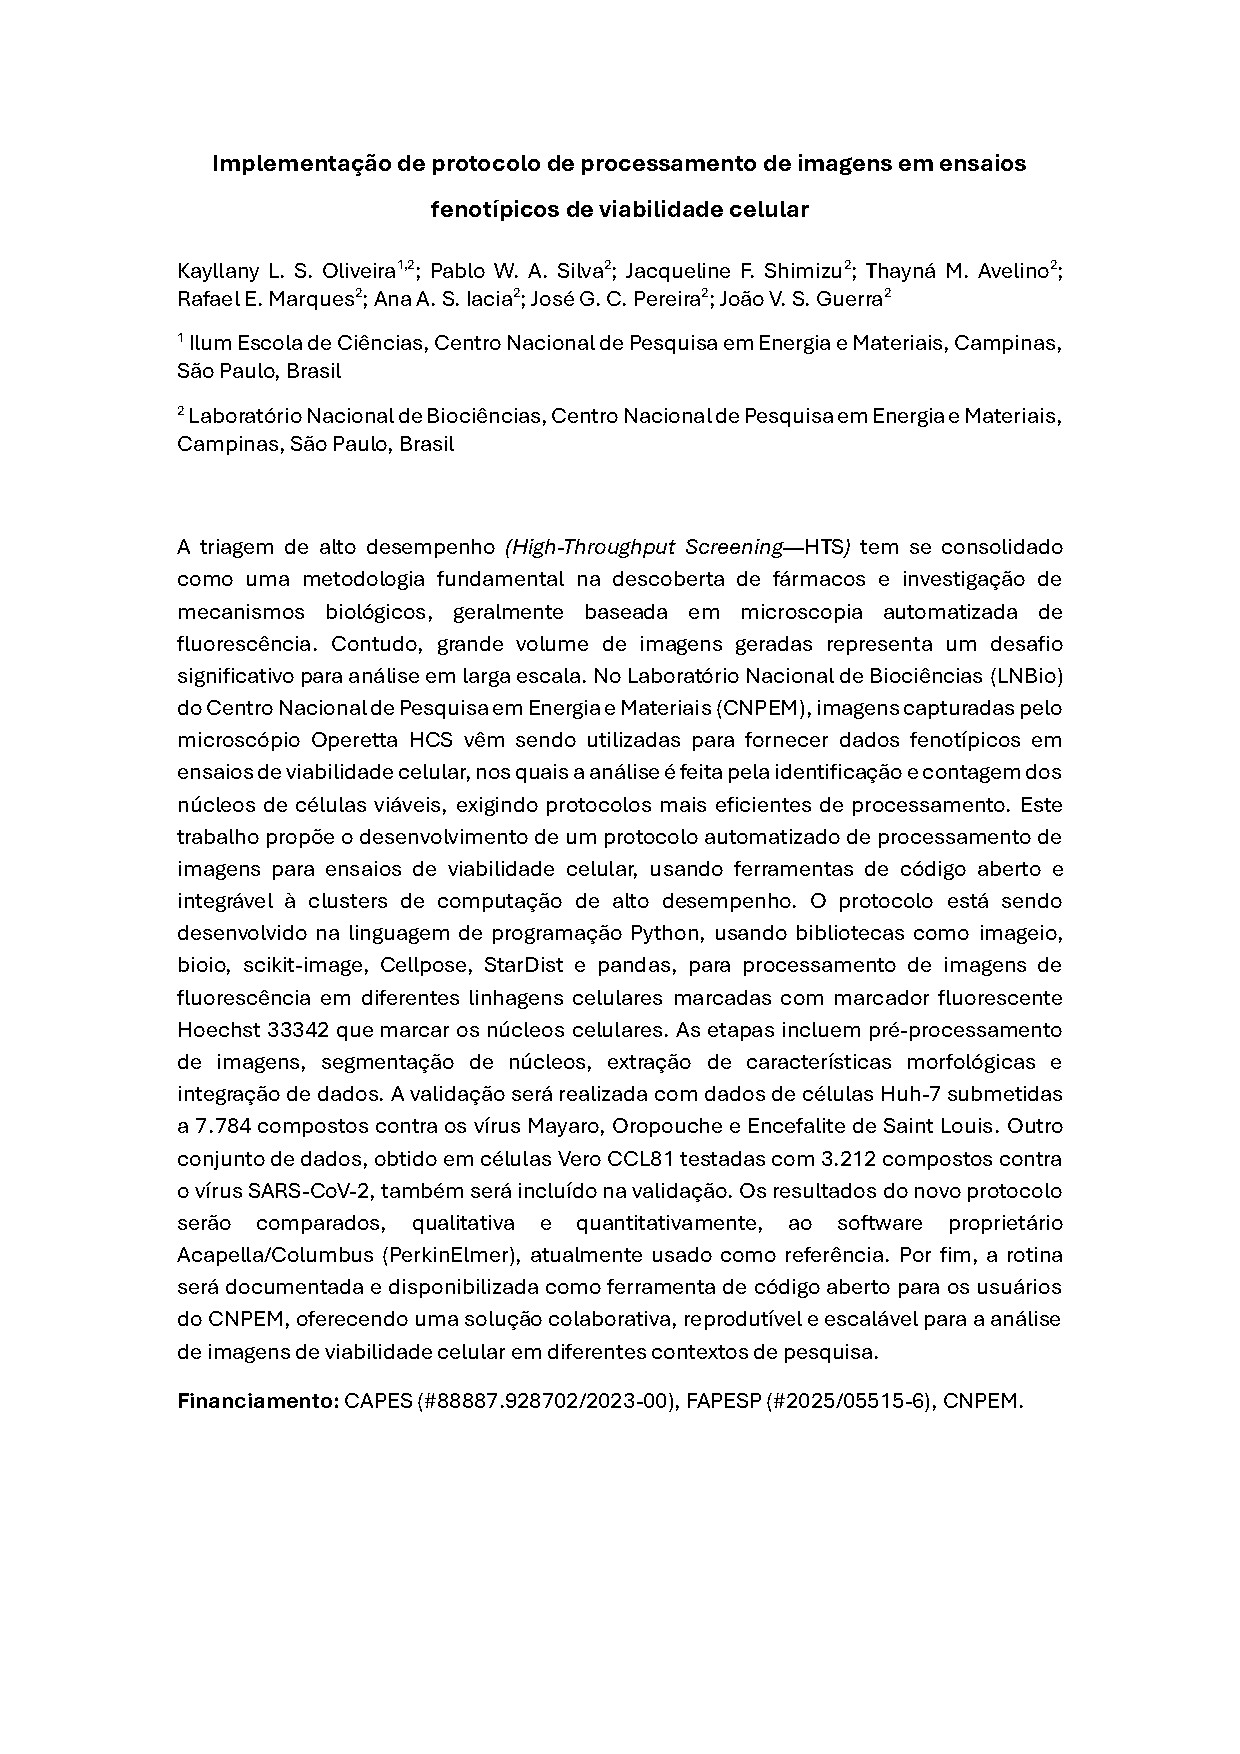
\includegraphics[width=0.9\textwidth]{attachments/[CEC VII] Resumo.pdf}
\end{figure}

\clearpage

\subsection{Pôster}

\begin{figure}[H]
 \centering
 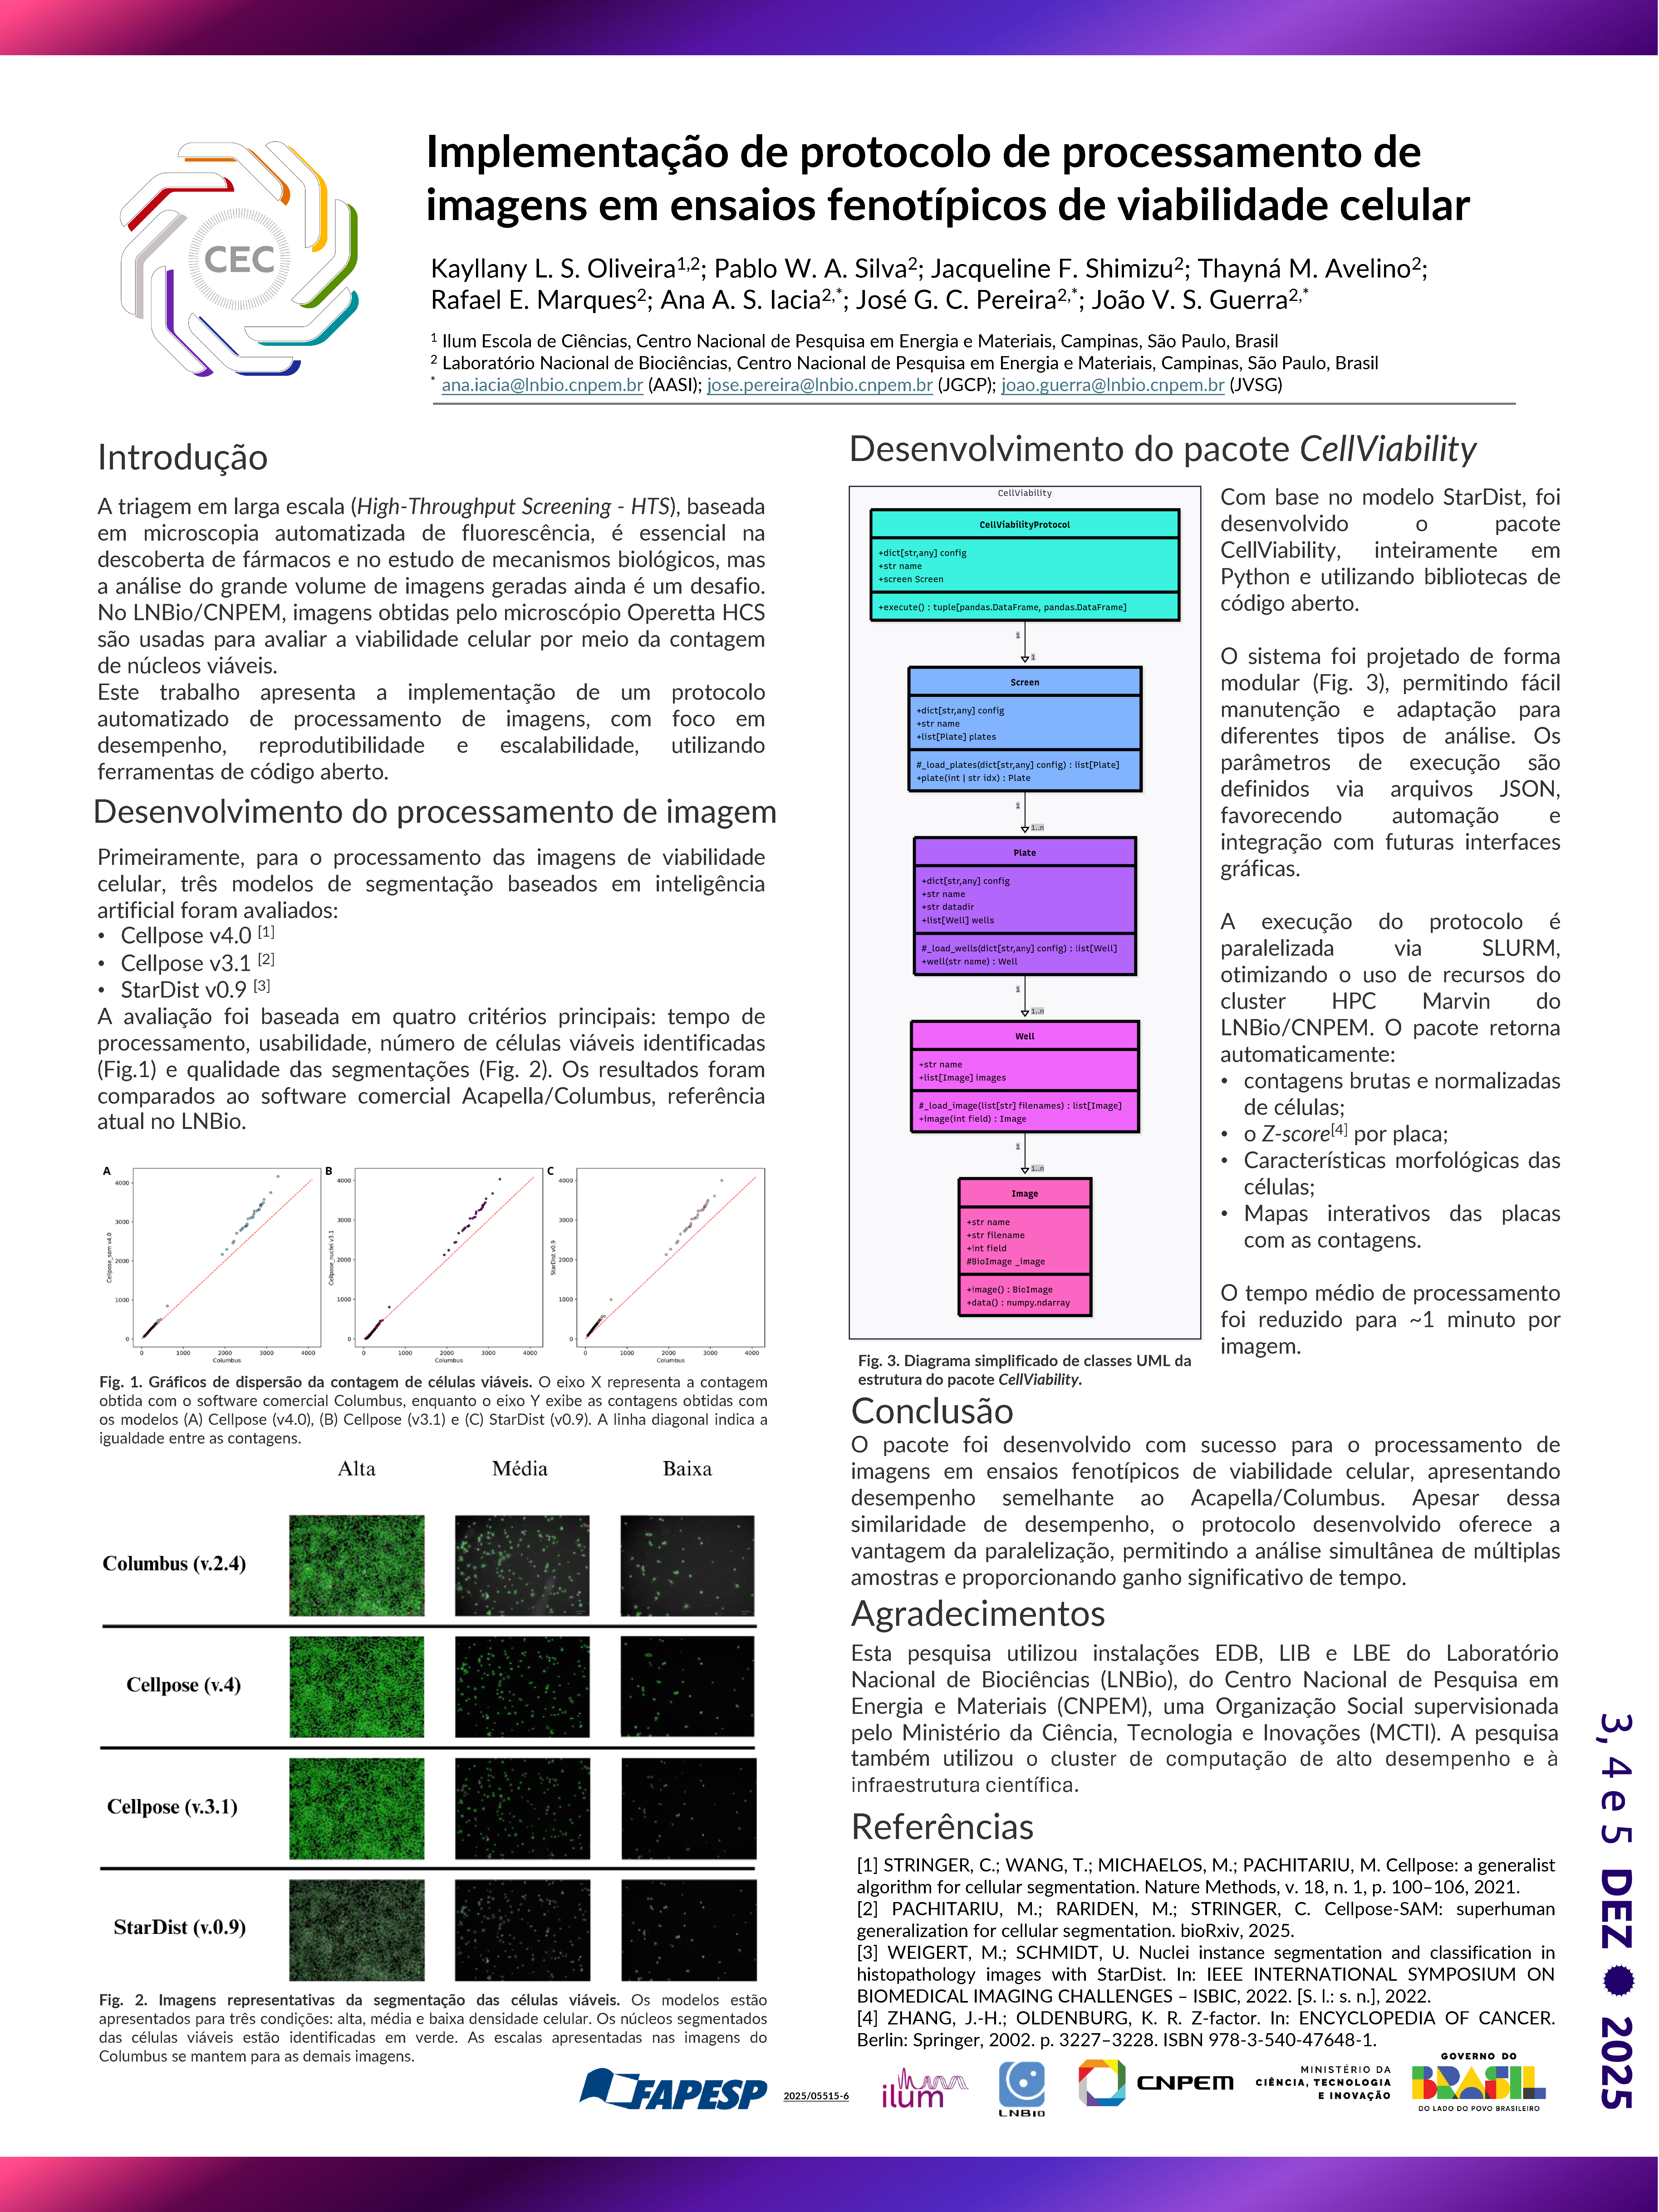
\includegraphics[width=\textwidth]{attachments/[CEC VII] Poster.pdf}
\end{figure}

\clearpage

\subsection{Flash talk}

\begin{figure}[H]
 \centering
 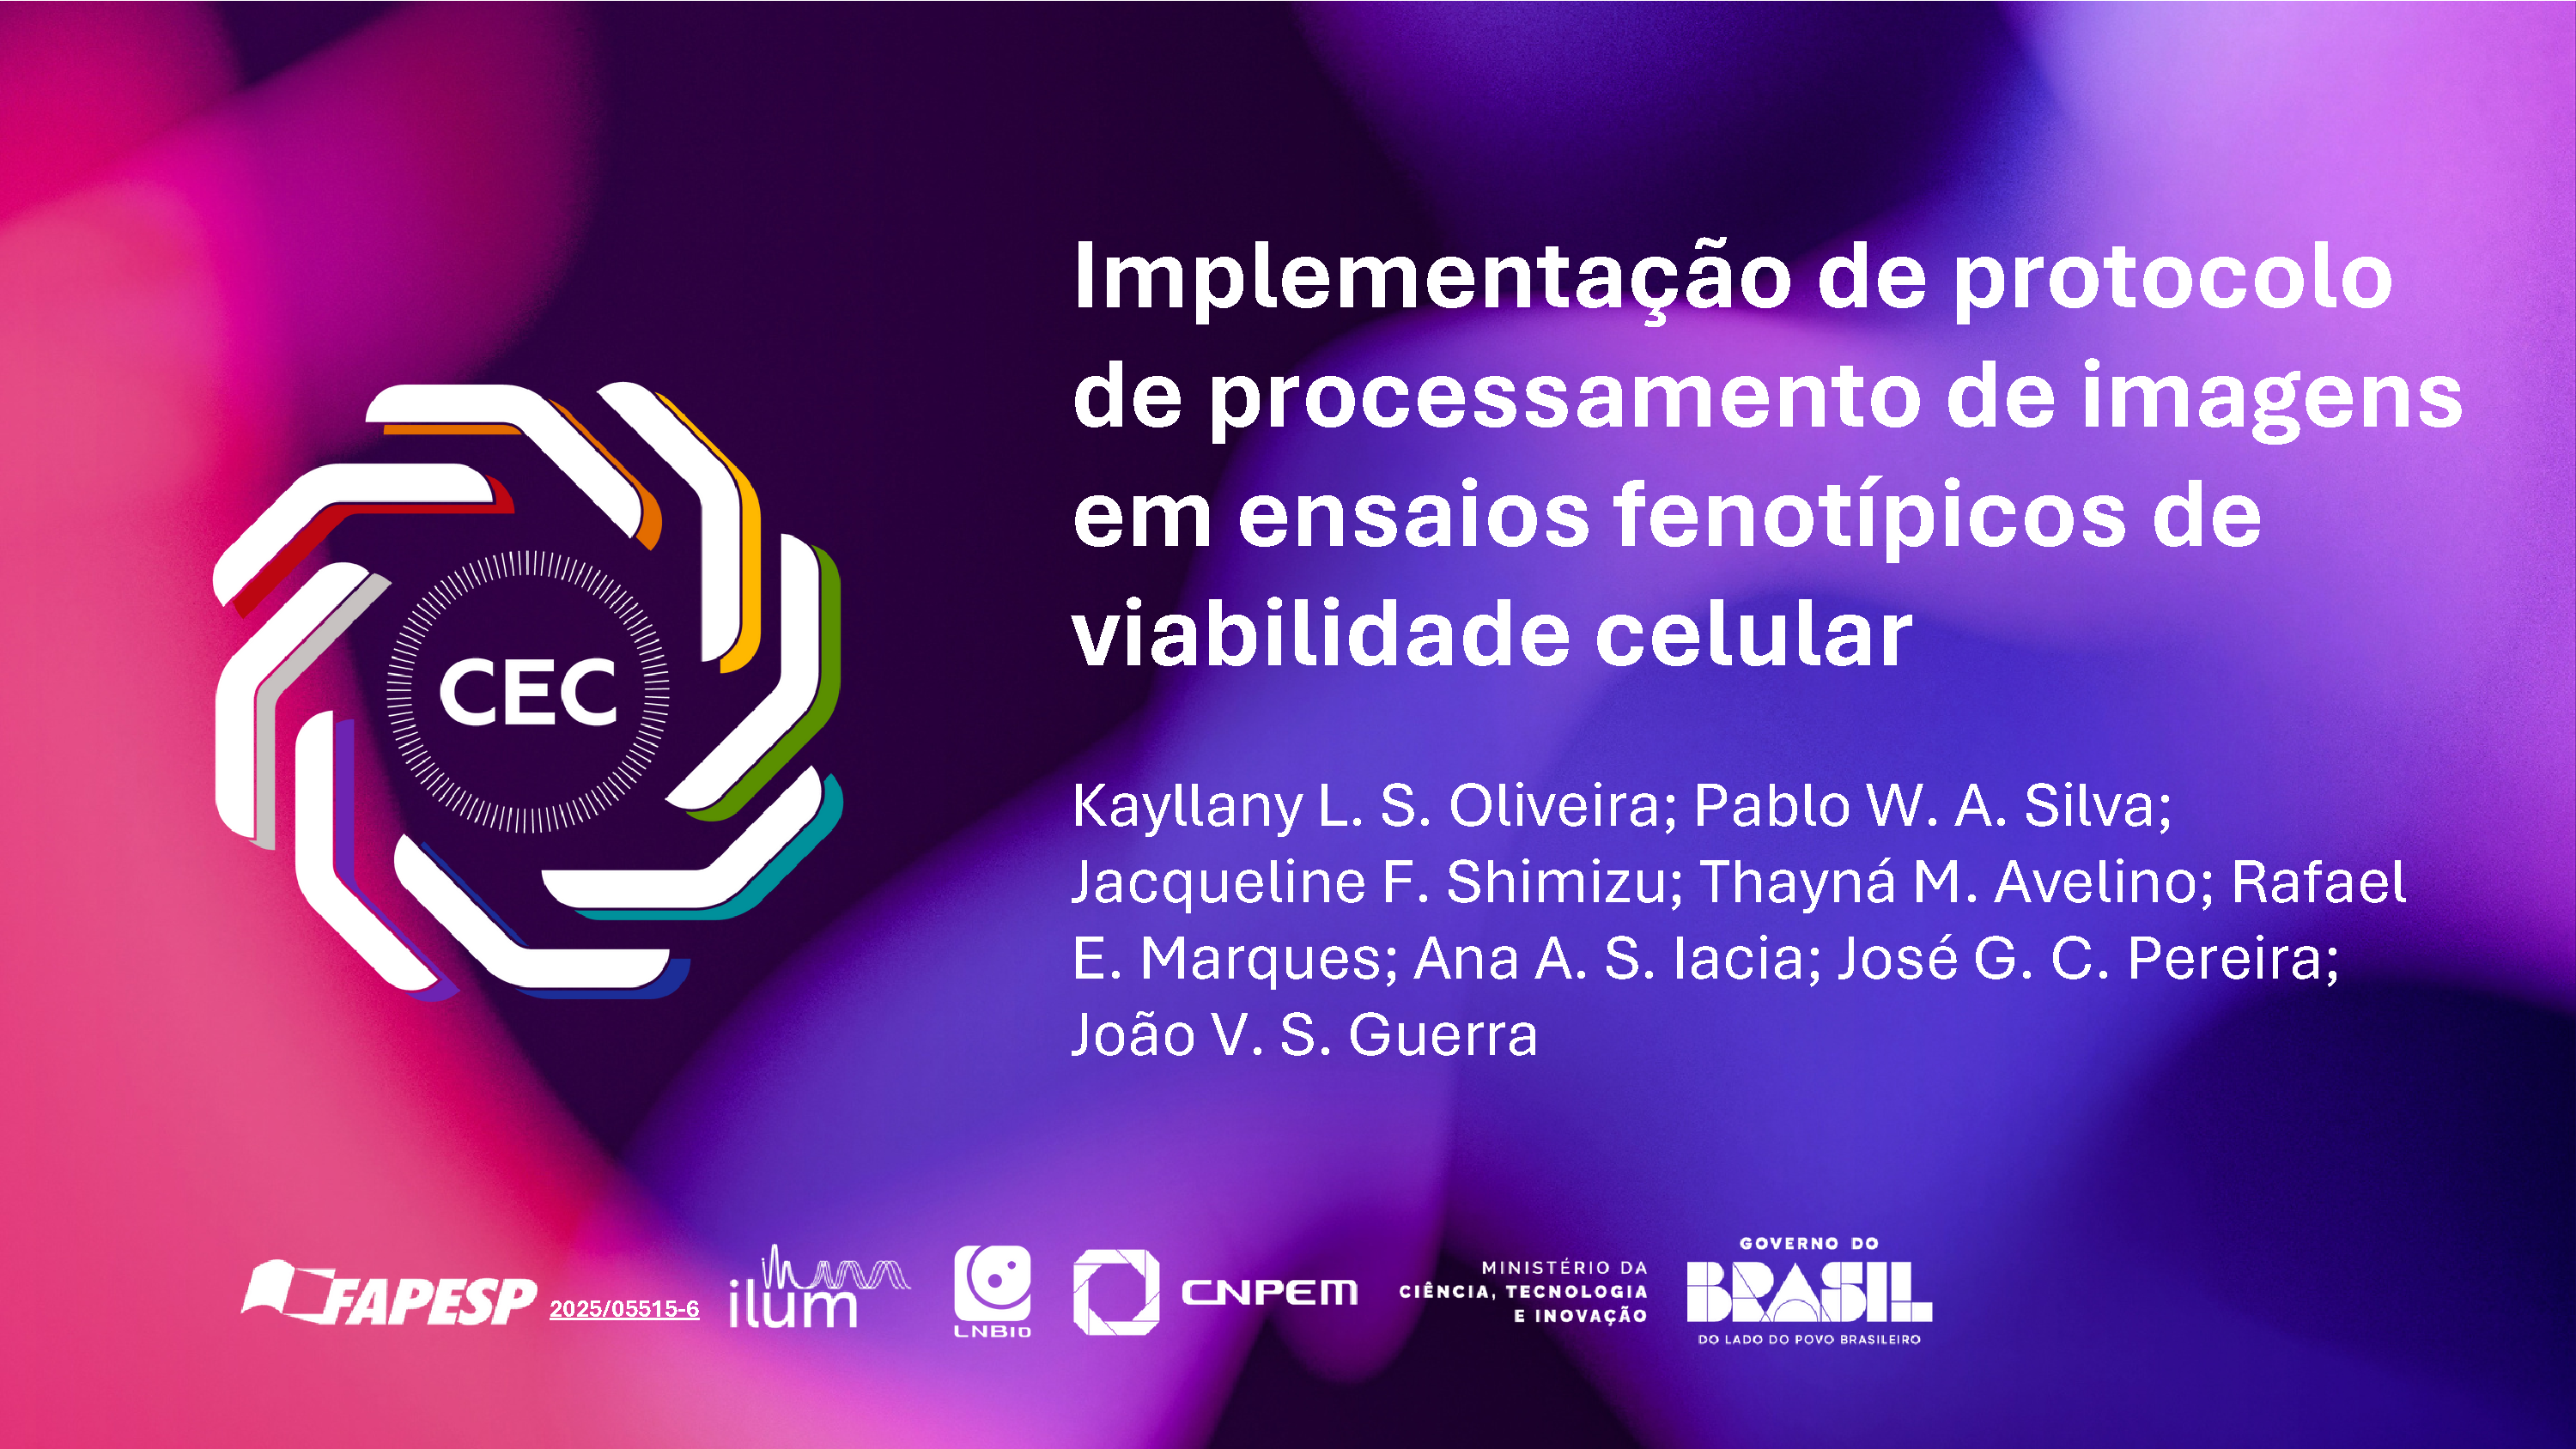
\includegraphics[page=1, width=\textwidth]{attachments/[CEC VII] Flash talk.pdf} \\
 \vspace{2cm}
 \includegraphics[page=2, width=\textwidth]{attachments/[CEC VII] Flash talk.pdf}
\end{figure}

\end{document}
